
%% This is file `elsarticle-template-1-num.tex',
%%
%% Copyright 2009 Elsevier Ltd
%%
%% This file is part of the 'Elsarticle Bundle'.
%% ---------------------------------------------
%%
%% It may be distributed under the conditions of the LaTeX Project Public
%% License, either version 1.2 of this license or (at your option) any
%% later version.  The latest version of this license is in
%%    http://www.latex-project.org/lppl.txt
%% and version 1.2 or later is part of all distributions of LaTeX
%% version 1999/12/01 or later.
%%
%% The list of all files belonging to the 'Elsarticle Bundle' is
%% given in the file `manifest.txt'.
%%
%% Template article for Elsevier's document class `elsarticle'
%% with numbered style bibliographic references
%%
%% $Id: elsarticle-template-1-num.tex 149 2009-10-08 05:01:15Z rishi $
%% $URL: http://lenova.river-valley.com/svn/elsbst/trunk/elsarticle-template-1-num.tex $
%%
\documentclass[preprint,12pt]{elsarticle}

%% Use the option review to obtain double line spacing
%% \documentclass[preprint,review,12pt]{elsarticle}

%% Use the options 1p,twocolumn; 3p; 3p,twocolumn; 5p; or 5p,twocolumn
%% for a journal layout:
%% \documentclass[final,1p,times]{elsarticle}
%% \documentclass[final,1p,times,twocolumn]{elsarticle}
%% \documentclass[final,3p,times]{elsarticle}
%% \documentclass[final,3p,times,twocolumn]{elsarticle}
%% \documentclass[final,5p,times]{elsarticle}
%% \documentclass[final,5p,times,twocolumn]{elsarticle}

%% if you use PostScript figures in your article
%% use the graphics package for simple commands
%% \usepackage{graphics}
%% or use the graphicx package for more complicated commands
%% \usepackage{graphicx}
%% or use the epsfig package if you prefer to use the old commands
%% \usepackage{epsfig}

%% The amssymb package provides various useful mathematical symbols
\usepackage{amssymb}
\usepackage{graphics}
\usepackage{url}
\usepackage{amsmath}
\usepackage{graphicx}
\usepackage{url}
\usepackage{theorem}
\usepackage{subfig}
\usepackage{amsfonts}
\usepackage{amssymb}
\usepackage{graphicx}
\usepackage{pstricks}
\usepackage{listings}
\usepackage{cancel}
%\usepackage[lined]{algorithm2e}
\usepackage{cmmib57}
\usepackage{array}
\usepackage{amssymb}

\usepackage[noend]{algorithmic}
\usepackage[boxed]{algorithm}
\usepackage{setspace}
\renewcommand{\algorithmicrequire}{\textbf{ALGORITHM}}
\floatname{algorithm}{Algorithm}

\usepackage{pst-tree}
\usepackage{lscape}
\usepackage{subfig}
\usepackage{verbatim}
\usepackage{multicol}

\newcommand{\band}{\mbox{ and }}
\newcommand{\true}{\mbox{true}}
\newcommand{\false}{\mbox{false}}
\newcommand{\dd}{\mathinner{\ldotp\ldotp}}
\newcommand{\cpos}{\textit{P}}      % cover positions
\newcommand{\carr}{\textsf{C}}      % cover array
\newcommand{\cmarr}{\textsf{C}^\mathrm{M}}      % maximal cover array
\newcommand{\sarr}{\textsf{LS}}      % left-seed array
\newcommand{\rsarr}{\textsf{RS}}      % right-seed array
\newcommand{\rsarrr}{\textsf{RS'}}      % RS' array
\newcommand{\smarr}{\textsf{LS}^\mathrm{M}}      % maximal left-seed array
\newcommand{\rsmarr}{\textsf{RS}^\mathrm{M}}      % maximal right-seed array
\newcommand{\parr}{\textsf{P}}      % period array
\newcommand{\barr}{\textsf{B}}      % period array
\newcommand{\rarr}{\textsf{R}}      % period array
\newcommand{\cv}{\textsf{CV}} 
\newcommand{\fl}{\textsf{FL}} 
\newcommand{\ON}{\mathit{ON}}
\newcommand{\firstappear}{\textit{First-appear}}
\newcommand{\delete}{\mathit{Delete}}
\newcommand{\Powers}{\mathit{Powers}}
\newcommand{\numbercheck}{\mathit{check}}
\newcommand{\Border}[1]{\ensuremath{\mathrm{Border}(#1)}}
\newcommand{\Per}[1]{\ensuremath{\mathrm{Per}(#1)}}

\newcommand{\mls}[1]{\ensuremath{\mathrm{mls}(#1)}}
\newcommand{\Mls}[1]{\ensuremath{\mathrm{Mls}(#1)}}
\newcommand{\mrs}[1]{\ensuremath{\mathrm{mrs}(#1)}}
\newcommand{\Mrs}[1]{\ensuremath{\mathrm{Mrs}(#1)}}

\newcommand{\Included}{\ensuremath{\mathrm{Included}}}
\newcommand{\ALS}{\ensuremath{\mathrm{ALS}}}

\newcommand{\cO}{\ensuremath{\mathcal{O}}}
\newcommand{\gaplist}{\ensuremath{\mathit{Gap}}}
\newcommand{\covervalue}{\ensuremath{\mathit{cover}}}
\newcommand{\firstvalue}{\ensuremath{\mathit{first}}}
\newcommand{\ypBigoh}{\mathcal{O}}
\newcommand{\BO}{\mathcal{O}}
\newcommand{\HRule}{\rule{\linewidth}{0.5mm}}

\newtheorem{theorem}{Theorem}[section]
\newtheorem{problem}{Problem}
\newtheorem{lemma}[theorem]{Lemma}
\newtheorem{proposition}[theorem]{Proposition}
\newtheorem{corollary}[theorem]{Corollary}

\newenvironment{proof}[1][Proof]{\begin{trivlist}
\item[\hskip \labelsep {\bfseries #1}]}{\end{trivlist}}
\newenvironment{definition}[1][Definition]{\begin{trivlist}
\item[\hskip \labelsep {\bfseries #1}]}{\end{trivlist}}
\newenvironment{example}[1][Example]{\begin{trivlist}
\item[\hskip \labelsep {\bfseries #1}]}{\end{trivlist}}
\newenvironment{remark}[1][Remark]{\begin{trivlist}
\item[\hskip \labelsep {\bfseries #1}]}{\end{trivlist}}

\long\def\symbolfootnote[#1]#2{\begingroup%
\def\thefootnote{\fnsymbol{footnote}}\footnote[#1]{#2}\endgroup} 

%% The amsthm package provides extended theorem environments
%% \usepackage{amsthm}

%% The lineno packages adds line numbers. Start line numbering with
%% \begin{linenumbers}, end it with \end{linenumbers}. Or switch it on
%% for the whole article with \linenumbers after \end{frontmatter}.
%% \usepackage{lineno}

%% natbib.sty is loaded by default. However, natbib options can be
%% provided with \biboptions{...} command. Following options are
%% valid:

%%   round  -  round parentheses are used (default)
%%   square -  square brackets are used   [option]
%%   curly  -  curly braces are used      {option}
%%   angle  -  angle brackets are used    <option>
%%   semicolon  -  multiple citations separated by semi-colon
%%   colon  - same as semicolon, an earlier confusion
%%   comma  -  separated by comma
%%   numbers-  selects numerical citations
%%   super  -  numerical citations as superscripts
%%   sort   -  sorts multiple citations according to order in ref. list
%%   sort&compress   -  like sort, but also compresses numerical citations
%%   compress - compresses without sorting
%%
%% \biboptions{comma,round}

% \biboptions{}

%\journal{Journal of Discrete Algorithms} 

\begin{document}

\begin{frontmatter}


\begin{center}


% Upper part of the page  

\textsc{\huge King's College London}\\[1.5cm]

\textsc{\LARGE Department of Informatics}\\[1.5cm]



% Title
\HRule \\[0.4cm]
{ \LARGE \bfseries Nine-Month Progress Report}\\[0.4cm]

\HRule \\[1.5cm]

$\;$\\
$\;$\\
$\;$\\
$\;$\\
$\;$\\
$\;$\\
$\;$\\
$\;$\\
$\;$\\
$\;$\\
$\;$\\
$\;$\\
$\;$\\
$\;$\\
$\;$\\
$\;$\\


\begin{multicols}{2}
\begin{flushleft}
\emph{Author:}\\
Michalis Christou\\
$\;$\\
$\;$\\
$\;$\\
\emph{Supervisors:} \\
Prof Costas Iliopoulos\\
Prof Maxime Crochemore\\
$\;$\\
\begin{flushright}
June 2011
\end{flushright}
\end{flushleft}
\end{multicols}
\end{center}



%---------%---------%---------%---------%---------%---------%---------%--------%

\begin{center}
\begin{abstract}

This report contains results that have been accepted in conference proceedings during the first nine months of my PhD. 
So far I have studied a lot around strings and problems around them. More specifically I am showing an $\cO(|y|)$ time algorithm that computes the minimal left-seed array of a given string $y$, an $\cO(|y|\log |y|)$ time algorithm that computes the minimal right-seed array of a given string $y$, and a linear-time solution to compute the maximal left-seed/right-seed array by detecting border-free prefixes of the given string. Additionally I am presenting a problem on trees, how to output all subtree repeats of a tree in linear time using a string representation of the tree. \\
\noindent\textbf{Keywords:} algorithms, strings, trees, periodicity, covers, seeds

\end{abstract}
\end{center}

%---------%---------%---------%---------%---------%---------%---------%--------%
\end{frontmatter}

\newpage
\noindent\begin{large}\textbf{Acknowledgments}\end{large}\\
Thanks are extended to my family which has always been close to me and to my supervisors, Prof Costas Iliopoulos and Prof Maxime Crochemore, for their continuous supervision and guidance through the completion of this report.
\newpage
\noindent\begin{large}\textbf{Disclaimer}\end{large}\\
I declare the following to be my own work, unless otherwise referenced, as defined by the University’s policy on plagiarism.\\
\textbf{Michalis Christou}

\newpage
\tableofcontents
\newpage

\section{Introduction}

Strings appear in many fields of Mathematics and Computer Science like
combinatorics on words, pattern matching, data compression and automata
theory (see~\cite{Lot01,Lot05}), because of their paramount importance
in several applications and their theoretical aspects.

Throught this report I am showing results around my research in strings that have been accepted in conference proceedings during the first nine months of my PhD. More specifically in Section \ref{sec LS-RS} I am showing some results around quasiperiodicity in strings, an $\cO(|y|)$ time algorithm that computes the minimal left-seed array of a given string $y$\cite{cpm_2011}, an $\cO(|y|\log |y|)$ time algorithm that computes the minimal right-seed array of a given string $y$\cite{COCOON_2011}, and a linear-time solution to compute the maximal left-seed/right-seed array by detecting border-free prefixes of the given string\cite{COCOON_2011,cpm_2011}. Additionally I am presenting a problem on trees in Section \ref{sec SR}, how to output all subtree repeats of a tree in linear time using a string representation of the tree\cite{SPIRE_2011}. Finally, I give some future proposals and a brief conclusion in Section \ref{sec:conclusion}.


\section{Left-seed and right-seed arrays}
\label{sec LS-RS}
\subsection{Introduction}

The notion of periodicity in strings is well studied in many fields like
combinatorics on words, pattern matching, data compression and automata
theory (see~\cite{Lot01,Lot05}), because it is of paramount importance
in several applications, not to talk about its theoretical aspects.

The concept of quasiperiodicity is a generalization of the notion
of periodicity, and was firstly defined by Apostolico and Ehrenfeucht in~\cite{162414}.
In a periodic repetition, the occurrences of the single periods do not overlap.
In contrast, the quasiperiods of a quasiperiodic string may overlap.
We call a factor $u$ of a nonempty string $y$ a cover of $y$, if every letter 
of $y$ is within some occurrence of $u$ in $y$. Note that we consider the \emph{aligned covers},
where the cover $u$ of $y$ needs to be a border (i.e. a prefix and a suffix) of $y$. 
\emph{Seeds} are regularities of strings strongly related to the notion of
cover. They were first defined and studied by Iliopoulos, Moore and Park in~\cite{Iliopoulos96}.
The notion of seed is an extension of the definition of a cover of a string, 
as it is a cover of a superstring of the word.

A fundamental problem is to find all the covers of a string $y$ of length $n$. 
Linear-time algorithms were given by Moore and Smyth in~\cite{moore1994optimal}, 
and by Li and Smyth in~\cite{cover_bill}. An $\cO(\log(\log n))$-time work-optimal parallel 
algorithm was given later by Iliopoulos and Park in~\cite{iliopoulos1996work}. 
The corresponding problem on seeds is of much higher algorithmic difficulty, 
and at the moment, no linear-time algorithm is known.
The fastest algorithm was given by Iliopoulos, Moore and Park in~\cite{Iliopoulos96}, running in $\cO(n\log n)$ time.

A close and also fundamental problem is that of computing the shortest (resp. longest) cover of every prefix of a string. 
This gives rise to the so-called {\em minimal cover} (resp. {\em maximal cover}) {\em array}.
An integer array $\carr$ is the minimal cover (resp. maximal cover) array of $y$, if $\carr[i]$
is the minimal (resp. maximal) length of covers of $y[0\dd i]$.

Apostolico and Breslauer, in~\cite{DBLP:conf/birthday/ApostolicoB97,DBLP:journals/ipl/Breslauer92},
gave an online linear-time algorithm for computing the minimal cover array of a string, using the algorithm by Knuth, Morris and Pratt, 
in~\cite{KMP}, for computing the period of every prefix of a string in linear time.
In addition, Li and Smyth, in~\cite{cover_bill}, provided an algorithm, having the same characteristics, for computing the 
maximal cover array of a given string; this algorithm gives also all the covers for every prefix of the string. 

A left seed of a string $y$ of length $n$, firstly defined in~\cite{cpm_2011}, is a prefix of $y$ that is a cover of a superstring of $y$. 
Similarly, a right seed of a string $y$, also firstly defined in~\cite{cpm_2011}, is a suffix of $y$ that is a cover of a superstring of $y$. 
An integer array $\sarr$ is the minimal left-seed (resp. maximal left-seed) array of $y$, if $\sarr[i]$
is the minimal (resp. maximal) length of left seeds of $y[0\dd i]$.
The minimal right-seed array (resp. maximal right-seed) $\rsarr$ is defined in a similar fashion.
These structures, apart from their own theoretical interest, they might also prove useful in finding faster algorithms for problems 
on seeds.

In this report we summarise our previous results obtained for the left-seed and the right-seed arrays: 
a linear-time algorithm for computing the minimal left-seed array of $y$\cite{cpm_2011}, a linear-time
solution for computing the maximal left-seed array of $y$\cite{cpm_2011}, an $\cO(n\log n)$ time algorithm for 
computing the minimal right-seed array of $y$\cite{COCOON_2011} and a linear-time solution for computing the maximal right-seed array of $y$\cite{COCOON_2011}. It is important to note that all of the proposed algorithms use linear auxiliary space.

%\begin{comment}
%In order to compute the length of the left seeds of all prefixes of the string we use Apostolico and Breslauer's algorithm for computing the minimal cover array of a string \cite{DBLP:conf/birthday/ApostolicoB97,DBLP:journals/ipl/Breslauer92}. Our algorithm that computes the minimal
%right-seed array of a given string in $\cO(n\log n)$ time uses a variant of the partitioning algorithm designed by Crochemore~\cite{C81} (see also~\cite{CL07}, Chapter 9). For the sake of completeness, we give a linear-time solution to compute the maximal left-seed array by detecting border-free prefixes of the given string. It is easy to see that the algorithm for computing the maximal right-seed array of a string is exactly the same. Additionally we reduce the problem of finding all the left/right seeds of a string in finding all the covers of a string in some range of the string.
%In order to achive that we use Li and Smyth's algorithm for computing the maximal cover array of a string\cite{cover_bill}, which gives us the covers of all prefixes of the string. 
%\end{comment}

The rest of the section is structured as follows.
%
In Subsection~\ref{sec:definitions}, we present the basic definitions used throughout
the report, and we define the problems solved.
%
In Subsection~\ref{sec:properties}, we prove some useful properties of left seeds, right seeds, and covers,
used later on for the design and analysis of the provided algorithms.
%
In Subsection~\ref{sec:algorithms}, we describe and analyse the proposed algorithms. %and in Section \ref{sec:experiments} we provide some experimental results, which verify the linear runtime of our algorithm that computes the left-seed array of a given string.
%
Finally, we give some future proposals and a brief conclusion in Section~\ref{sec:conclusion}.

%---------%---------%---------%---------%---------%---------%---------%--------%

\subsection{Definitions and Problems}\label{sec:definitions}

Throughout this report we consider a string $y$ of length $|y| = n$, $n>0$, on a
fixed alphabet. It is represented as $y[0\dd n-1]$.
A string $w$ is a {\em factor} of $y$ if $y=uwv$ for two strings $u$ and $v$.
It is a {\em prefix} of $y$ if $u$ is empty and a {\em suffix} of $y$
if $v$ is empty.
The concatenation of two strings $x$ and $y$ is the string of the letters of $x$ followed by the letters of $y$. 
It is denoted by $xy$.
A string $u$ is a \textit{border} of $y$ if $u$ is a both a prefix and a suffix of $y$.
{\em The border} of $y$, denoted by $\Border{y}$,  is the length of the longest border of $y$.
The {\em border array} $\barr$ of $y$ is the array of integers $\barr[0 \dd n-1]$
for which $\barr[i]$, $0\leq i < n$, stores the length of the border of the prefix $y[0 \dd i]$.
A string $u$ is a \textit{period} of $y$ if $y$ is a prefix of $u^k$ for
some positive integer $k$, or equivalently if $y$ is a prefix of $uy$.
{\em The period} of $y$, denoted by $\Per{y}$, is the length of the shortest period of $y$.
It is a known fact that, for any string $y$, $\Per{y} + \Border{y} = |y|$.
The {\em period array} $\parr$ of $y$ is the array of integers $\parr[0 \dd n-1]$
for which $\parr[i]$, $0\leq i < n$, stores the length of the period of the prefix $y[0 \dd i]$.
For a string $u=u[0\dd m-1]$ such that $u$ and $v$ share a common part
 $u[m-\ell \dd m-1]=v[0\dd \ell-1]$ for some $1 \leq \ell \leq m$, the string
 $u[0\dd m-1]v[\ell\dd n-1]=u[0\dd m-\ell-1]v[0 \dd n-1]$ is called
 a {\em superposition} of $u$ and $v$ with an \textit{overlap} of length $\ell$.
A string $x$ of length $m$ is a {\em cover} of $y$ if both
$m<n$ and there exists a set of positions $\cpos \subseteq \{0, \ldots, n-m\}$
that satisfies both $y[i\dd i+m-1]=x$ for all $i\in \cpos$ and
$\bigcup_{i\in \cpos} \{ i,\ldots,i+m-1 \} = \{0,\ldots,n-1\}$.
The {\em minimal cover array} $\carr$ of $y$ is the array of integers $\carr[0 \dd n-1]$
for which $\carr[i]$, $0\leq i < n$, stores the length of the
shortest cover of the prefix $y[0 \dd i]$.
The {\em maximal cover array} $\carr$ of $y$ is the array of integers $\carr[0 \dd n-1]$
for which $\cmarr[i]$, $0\leq i < n$, stores the length of the longest cover of the prefix $y[0 \dd i]$ which is smaller than $y$ ($0$ if none).

A string $v$ is a \emph{seed} of $y$, if it is a cover
of a superstring of $y$. A left seed of a string $y$ is a prefix of $y$ that it is
a cover of a superstring of $y$ of the form $yv$, where $v$ is a possibly empty string.
The {\em minimal left seed} of $y$, denoted by $\mls{y}$, is the shortest prefix of $y$ that is a cover of a superstring of $y$.
The {\em minimal left-seed array} $\sarr$ of $y$ is the array of integers $\sarr[0 \dd n-1]$
for which $\sarr[i]$, $0\leq i < n$, stores the length of the minimal left seed of the prefix $y[0 \dd i]$.
The {\em maximal left seed} of $y$, denoted by $\Mls{y}$, is the longest prefix of $y$ that is a cover of a superstring of $y$.
The {\em maximal left-seed array} $\smarr$ of $y$ is the array of integers $\smarr[0 \dd n-1]$
for which $\smarr[i]$, $0\leq i \leq n-1$, stores the length of the maximal left seed of the prefix $y[0 \dd i]$, 
which is smaller than $i+1$ (0 if none).
The {\em minimal right seed} of $y$, denoted by $\mrs{y}$, is the shortest suffix of $y$ that is a cover of a superstring of $y$.
The {\em minimal right-seed array} $\rsarr$ of $y$ is the array of integers $\rsarr[0 \dd n-1]$
for which $\rsarr[i]$, $0\leq i < n$, stores the length of the minimal right seed of the prefix $y[0 \dd i]$.
The {\em maximal right seed} of $y$, denoted by $\Mrs{y}$, is the longest suffix of $y$ that is a cover of a superstring of $y$.
The {\em maximal right-seed array} $\rsmarr$ of $y$ is the array of integers $\rsmarr[0 \dd n-1]$
for which $\rsmarr[i]$, $0\leq i \leq n-1$, stores the length of the maximal left seed of the prefix $y[0 \dd i]$, 
which is smaller than $i+1$ (0 if none).

The following example  shows $\barr$, $\parr$, $\carr$, $\cmarr$, $\sarr$, $\smarr$, $\rsarr$, and $\rsmarr$ for the 
string $y=\texttt{abaababaabaabab}$ and all its left and right seeds. \\

\parbox{\textwidth}{\centering
\small
\tabcolsep0mm\begin{tabular}[t]{@{}r@{\quad}*{15}{c}@{}}\hline
$i$ & \makebox[4.5mm]{0}& \makebox[4.5mm]{1}&
\makebox[4.5mm]{2}& \makebox[4.5mm]{3}& \makebox[4.5mm]{4}&
\makebox[4.5mm]{5}& \makebox[4.5mm]{6}& \makebox[4.5mm]{7}&
\makebox[4.5mm]{8}& \makebox[4.5mm]{9}& \makebox[4.5mm]{10}&
\makebox[4.5mm]{11}& \makebox[4.5mm]{12}& \makebox[4.5mm]{13}& \makebox[4.5mm]{14}\\
\hline
$y[i]$&\texttt{a}&\texttt{b}&\texttt{a}&\texttt{a}&\texttt{b}&\texttt{a}&\texttt{b}&\texttt{a}&\texttt{a}&\texttt{b}&\texttt{a}&\texttt{a}&\texttt{b}&\texttt{a}&\texttt{b}\\
$\barr[i]$&0&0&1&1&2&3&2&3&4&5&6&4&5&6&7\\
$\parr[i]$&1&2&2&3&3&3&5&5&5&5&5&8&8&8&8\\
$\carr[i]$&1&2&3&4&5&3&7&3&9&5&3&12&5&3&15\\
$\cmarr[i]$&0&0&0&0&0&3&0&3&0&5&6&0&5&6&0\\
$\sarr[i]$&1&2&2&3&3&3&3&3&3&3&3&3&3&3&13\\
$\smarr[i]$&0&0&2&3&4&5&6&7&8&9&10&11&12&13&14\\
$\rsarr[i]$&1&2&2&3&3&3&5&3&5&5&3&8&5&3&8\\
$\rsmarr[i]$&0&0&2&3&4&5&6&7&8&9&10&11&12&13&14\\ \hline
\end{tabular}
}

\bigskip
\textbf{All left seeds of $y$:} $\texttt{aba}$, $\texttt{abaaba}$, $\texttt{abaababa}$, $\texttt{abaababaa}$, 
$\texttt{abaababaab}$, $\texttt{abaababaaba}$, $\texttt{abaababaabaa}$, $\texttt{abaababaabaab}$, $\texttt{abaababaabaaba}$, 
$\texttt{abaababaa}$\\$\texttt{baabab}$

\bigskip
\textbf{All right seeds of $y$:} $\texttt{aabaabab}$, $\texttt{baabaabab}$, $\texttt{abaabaabab}$,
$\texttt{babaabaabab}$, $\texttt{ababaabaabab}$,$\texttt{aababaabaabab}$, $\texttt{baababaabaabab}$, $\texttt{abaababaabaabab}$

\bigskip
We consider the following problems for a given string $y$.
%
\begin{problem}[Computing all left seeds]
\label{problem all ls}
Compute all the left seeds of $y$.
\end{problem}
%
\begin{problem}[Computing all right seeds]
\label{problem all rs}
Compute all the right seeds of $y$.
\end{problem}
%
\begin{problem}[Computing the minimal left-seed array]
\label{problem min LS}
Compute the minimal left-seed array $\sarr$ of $y$.
\end{problem}
%
\begin{problem}[Computing the maximal left-seed array]
\label{problem max LS}
Compute the maximal left-seed array $\smarr$ of $y$.
\end{problem}
%
\begin{problem}[Computing the minimal right-seed array]
\label{problem min RS}
Compute the minimal right-seed array $\rsarr$ of $y$.
\end{problem}
%
\begin{problem}[Computing the maximal right-seed array]
\label{problem max RS}
Compute the maximal right-seed array $\rsmarr$ of $y$.
\end{problem}


%---------%---------%---------%---------%---------%---------%---------%--------%

\subsection{Properties}\label{sec:properties}

In this subsection, we prove some useful properties of left seeds, of right seeds, and of covers of a given string $y$. 

%The following lemma gives the necessary and sufficient condition for a prefix of a string to be a left seed of that string, 
%a similar proof is given in~\cite{cpm_2011}.

\begin{lemma}[\cite{cpm_2011}]
\label{lem:1}
A string $z$ is a left seed of $y$ iff it covers a prefix of $y$ whose length is at least the period of $y$.
\label{lemma ls condition}
\end{lemma}
\begin{proof}
Direct: Suppose a string $z$ covers a prefix of $y$, say $uv$, larger or equal to $\Per{y}$, where $|u|=\Per{y}$ and $v$ is
a possibly non empty string. Let $k$ the smallest integer such that $y$ is a prefix of $u^{k}$. 
Then $z$ is a cover of $u^{k}v=ywv$, for some string $w$, possibly empty. Therefore $z$ is a left seed of $y$.

\noindent Reverse: Let $z$ a left seed of $y$.
\begin{itemize}
 \item if $|z|\leq \Border{y}$. Then a suffix $v$ of $z$, possibly empty, is a prefix of the border (consider the left seed that covers 
 $y[\Per{y}-1]$). Then $z$ is a cover of $uv$, where $u$ is the period of $y$.
 \item if $|z| > \Border{y}$. Let $z$ not a cover of a prefix of $y$ larger or equal to $\Per{y}$.
Let $v$ a border of $y$ such that $|v| = \Border{y}$. Then $v$ is a factor of $z$, such that $z=uvw$, where $u$ and $w$
are non empty words (consider the left seed that covers $y[\Per{y}-1]$). This gives $uv$ a longest border for $y$, which is a contradiction.\qed
\end{itemize}
\end{proof}

\begin{lemma}[\cite{COCOON_2011}]
A string $z$ is a right seed of $y$ iff it covers a suffix of $y$ whose length is at least the period of $y$.
\label{lemma rs condition}
\end{lemma}
\begin{proof}
Direct consequence of Lemma~\ref{lemma ls condition}.\qed
\end{proof}

\begin{lemma}[\cite{moore1994optimal}]
Let $u$ be a proper cover of $x$, in our case some prefix $y[0\dd i]$ of $y$, and let $z\neq u$ be a substring of $x$ such that $|z|\leq |u|$. 
Then $z$ is a cover of $x$ if and only if $z$ is a cover of $u$.
\label{lemma cover of a cover}
\end{lemma}
\begin{proof}
Clearly if $z$ is a cover of $u$ and $u$ a cover of $x$ then $z$ is a cover of $x$. 
Suppose now that both $z$ and $u$ cover $x$. Then $z$ is a border of $x$ and hence of $u$ ($|z|\leq |u|$); 
thus $z$ must also be a cover of $u$.\qed
\end{proof}



\begin{lemma}[\cite{cpm_2011}]
\label{lemma ls aperiodic}
Let $y$ a string of length $n$ and $\Per{y} = n$, then the minimal left seed of $y$ is $y$.
\end{lemma}
\begin{proof}
By definition of the minimal left seed: $|\mls{y}|\leq n$. Let $|\mls{y}| < n$. Then, in order to
cover $y$, a non-empty prefix of $\mls{y}$, say $w$, is a suffix of $y$ (consider the left seed that covers $y[n-1]$).
Then $n-|w|$ gives a shorter period for $y$, which is a contradiction.\qed
\end{proof}

\begin{lemma}[\cite{cpm_2011}]
\label{lemma LS[i]<=LS[i+1]}
Let $\sarr[i]=|\mls{y[0 \dd i]}|$, for all $0 \leq i < n$, then $\sarr[i] \leq \sarr[i+1]$, for all $0 \leq i < n-1$.
\end{lemma}
\begin{proof}
Let $\sarr[i] > \sarr[i+1]$. By definition of the minimal left seed: $\sarr[i]$ covers some superstring $y[0 \dd i]u$, where $u$ is a
possibly empty string, and $\sarr[i+1]$ covers some superstring $y[0 \dd i+1]v$, where $v$ is a possibly empty string.
In other words $\sarr[i+1]$ covers $y[0 \dd i]y[i+1]v$. Therefore, by definition of the minimal left seed, $\sarr[i+1]$ is a minimal left seed of $y[0 \dd i]$. But then we get a shorter left seed for $y[0 \dd i]$, which is a contradiction.\qed
\end{proof}

\begin{lemma}[\cite{cpm_2011}]
\label{lemma max ls}
Let $y$ a string of length $n$ and $\Per{y} = k$, then
\begin{itemize}
 \item if $k=n$, then there is no maximal left seed for $y$
 \item if $k<n$, then the maximal left seed of $y$ is $y[0\dd n-2]$
\end{itemize}
\end{lemma}
\begin{proof}
\begin{itemize}
 \item if $k=n$, then, by definition of the maximal left seed, it holds that $|\mls{y}| < n$. Let $y[0\dd j]$ be the maximal
left seed of $y$, with $0 \leq j < n$. Then, in order to cover $y$, a non-empty prefix of $y[0 \dd j]$, say $w$, 
is a suffix of $y$ (consider the maximal left seed that covers $y[n-1]$). Then $n-|w|$ gives a shorter period for $y$, which is a contradiction.
 \item if $k<n$, then the maximal left seed of $y$ is $y[0..n-2]$, as it is a cover of the superstring $yy[\Border{y}\dd n-2]$ of $y$,
and it has the maximum length allowed, which is $n-1$. \qed
\end{itemize}
\end{proof}

\begin{lemma}[\cite{COCOON_2011}]
\label{lemma max rs}
Let $y$ a string of length $n$ and $\Per{y} = k$, then
\begin{itemize}
 \item if $k=n$, then there is no maximal right seed for $y$.
 \item if $k<n$, then the maximal right seed of $y$ is $y[1..n-1]$
\end{itemize}
\end{lemma}
\begin{proof}
Similar to the proof of Lemma~\ref{lemma max ls}. \qed
\end{proof}


%---------%---------%---------%---------%---------%---------%---------%--------%

\subsection{The algorithms}\label{sec:algorithms}

In this subsection, we describe our algorithms for solving Problems~\ref{problem all ls}-\ref{problem max RS} for a string $y$ of length $n$.

\subsubsection{Computing the minimal and the maximal left-seed array}

In this subsection, we describe our algorithms for solving Problem~\ref{problem min LS} and Problem~\ref{problem max LS}.
For solving Problem~\ref{problem min LS}, we use the algorithm for computing the minimal cover array by Apostolico and 
Breslauer~\cite{DBLP:conf/birthday/ApostolicoB97,DBLP:journals/ipl/Breslauer92} in linear time, and Lemma~\ref{lem:1}, which gives
the necessary and sufficient condition for a prefix of a string to be a left seed of that string.
Problem~\ref{problem max LS} reduces to detecting border-free prefixes of the given string.

Algorithm {\sc R-Array} computes an array $\rarr$, which stores the length of the longest prefix of $y$ that is covered
by $y[0\dd i]$, $0$ if none. It takes as input the minimal cover array $\carr$.

    \begin{algorithm}
      %\caption{\label{algo:R-array}
       % Computation of R-array of a string $y$ of length $n$.  }
      \begin{algorithmic}[1]
        \REQUIRE {\sc R-Array}($\carr$, $n$)
        \STATE \textbf{for } $i\leftarrow0$ \textbf{to } $n-1$ \textbf{do }$\rarr[i]\leftarrow0$;
        \STATE \textbf{for } $i\leftarrow0$ \textbf{to } $n-1$ \textbf{do }$\rarr[\carr[i]-1] \leftarrow i+1$;
        \RETURN $\rarr[0 \dd n-1]$;
      \end{algorithmic}
    \end{algorithm}

Algorithm {\sc Minimal-Left-Seed-Array} computes an array $\sarr$, which stores the length
of the minimal left seed of $y[0\dd i]$. It takes as input the array $\rarr$ and the period array $\parr$.


    \begin{algorithm}
     % \caption{\label{algo:lseed-array2}
      %  Computation of minimal left seed array $\LSeed[1 \dotdot n]$ of a string $y$ of length $n$.}
      \begin{algorithmic}[1]
        \REQUIRE {\sc Minimal-Left-Seed-Array}($y$, $n$, $\parr$,$\rarr$)
        \STATE{\textbf{for } $i\leftarrow0$ \textbf{to } $n-1$ \textbf{do }}
        \STATE{\textbf{\quad if } $\parr[i]\leftarrow i+1$ \textbf{do } $\sarr[i]\leftarrow i+1$;}
        \STATE{\textbf{\quad else}}
	       \STATE{\text{\quad \quad}$ls\leftarrow \sarr[i-1]$};
                   \STATE \textbf{\quad \quad while } $\rarr[ls-1]< \parr[i]$ \textbf{do } $ls\leftarrow ls+1$;
		   \STATE{\text{\quad \quad}$\sarr[i]\leftarrow ls$};
        \RETURN $\sarr[0 \dd n-1]$;
      \end{algorithmic}
    \end{algorithm}

Then, we proceed to compute the array $\sarr$. There are two cases:

\begin{itemize}
 \item if $\parr[i]=i+1$, then by Lemma~\ref{lemma ls aperiodic}, $\sarr[i]=i+1$
 \item if $\parr[i]<i+1$, then by Lemma~\ref{lemma LS[i]<=LS[i+1]}, we must look for $\sarr[i]$ in the set $\{\sarr[i-1],...,n\}$
\end{itemize}

Lemma~\ref{lemma ls condition} gives the necessary and sufficient condition $(\rarr[ls-1] \geq \parr[i])$, i.e. the length of the 
longest prefix of $y$ that is covered by $y[0\dd ls-1]$ to be greater or equal than the period of $y[0\dd i]$, where $ls$ is the candidate 
length of the minimal left seed of $y[0\dd i]$.

\begin{theorem}
\label{main_theorem}
Computing the minimal left-seed array of a string $y$ of length $n$ can be done in linear time.
\label{thm:0}
\end{theorem}

\begin{proof}
Arrays $\carr$, $\parr$ and $\rarr$ can be computed in linear time as of~\cite{CL07,KMP,DBLP:conf/birthday/ApostolicoB97,DBLP:journals/ipl/Breslauer92}.
Then, we only have to prove that the process to compute array $\sarr$ runs in linear time,
as well. Let $c_{i}$ be the number of comparisons done in the second loop at step $i$. Then clearly,\\
$\textit{T=Time needed}$\\
$=2n+2+\sum^{n-1}_{i=0}(1+I(\parr[i]=i+1)+I(\parr[i]\neq i+1)*(2+2c_{i}-1))$\\
$=2n+2+\sum^{n-1}_{i=0} (2+I(\parr[i]\neq i+1)*2c_{i})$\\
$=2n+2+2n +I(\parr[i]\neq i+1) \sum^{n-1}_{i=0}2c_{i}$\\
Therefore
\begin{equation}
T \leq 4n+2+2\sum^{n-1}_{i=0}c_{i}
\label{eq:1}
\end{equation}

Let $s_{i}$ be the set of values checked in the second loop at step $i$. Clearly  $s_{i} \cap s_{i+1} = 1$ given by the 1st value
to be checked in $s_{i+1}$, which is the same as the last value in $s_{i}$. Then
\begin{equation}
c_{i} + c_{i+1}= |s_{i}| + |s_{i+1}| = |s_{i} \cup s_{i+1}| +  |s_{i} \cap s_{i+1}|\\
\end{equation}

\begin{equation}
c_{i} + c_{i+1}= |s_{i} \cup s_{i+1}| +  1
\label{eq:2}
\end{equation}

By Equations \ref{eq:1} and \ref{eq:2}:

\begin{equation}
T \leq 4n+2+2(n-1+|\bigcup^{n-1}_{i=0}s_{i}| )
\label{eq:3}
\end{equation}

As $\bigcup^{n-1}_{i=0}s_{i}$ is at most $\{0,...,n-1\}$ then $|\bigcup^{i=0}_{n-1}s_{i}| \leq n$, and so $T \leq 8n$.
Therefore $T=\cO(n)$. \qed
\end{proof}


For solving Problem~\ref{problem max LS}, we can use Lemma~\ref{lemma max ls} to obtain the following two cases.

\begin{itemize}
 \item if $\parr[i]=i+1$, then $\smarr[i]=0$
 \item if $\parr[i]<i+1$, then $\smarr[i]=i$
\end{itemize}

Hence, we obtain the following result.

\begin{theorem}
Computing the maximal left-seed array of a string $y$ of length $n$ can be done in linear time.
\end{theorem}


\subsubsection{Computing the minimal and the maximal right-seed array}

In this subsection, we describe our algorithms for solving Problem~\ref{problem min RS} and Problem~\ref{problem max RS}.
For solving Problem~\ref{problem min RS}, we use a variant of the partitioning algorithm in~\cite{C81,Iliopoulos96} to 
find the sets of ending positions of all the occurrences of each factor in the string. We are then able to find which suffix of each 
prefix of the string is covered by that factor, and check for right seeds using Lemma~\ref{lemma rs condition}. 
Problem~\ref{problem max RS} reduces to detecting border-free prefixes of the given string.

In the following lines, we give a brief description of the partitioning algorithm used for solving Problem~\ref{problem min RS}.

For a factor $w$ in $y$, the set of end positions of all the occurrences of $w$ in $y$, gives us the \emph{end set} of $w$.
We define an equivalence relation $\approx_{\ell}$ on positions of $y$ such that $i\approx _{\ell}j$ iff $y[i-\ell+1\dd i]=y[j-\ell+1\dd j]$.
Therefore, depending on the length of the factor, we get equivalence classes for each length $\ell$, $1\leq \ell \leq n$.
Equivalence classes for $\ell=1$ are found by going over $y$ once, and keeping the occurrences of each letter in separate sets.
For larger $\ell$, we consider classes of the previous level to make a refinement on them, and calculate the classes of that level.
So on level $\ell$, $1<\ell\leq n$, we refine a class $C$ by a class $D$, by splitting $C$ in classes $\{i\in C/i-1\in D\},\{i\in C/i-1 \notin D\}$.
In order to achieve a good running time, we do not use all classes for refinement; only classes of the previous level, which were split two
levels before, are used. From those, we can omit the largest siblings of each family, and use only the small ones for
the computation. We terminate the algorithm when all classes reach a singleton stage.

In Fig.~\ref{fig:tree}, the classes of $\approx_{\ell}$, ${\ell}=1,2,\ldots,8$, for the
string $y=\texttt{abaababaa}$\\$\texttt{baabab}$ are illustrated. The partitioning algorithm creates two types of sets at each round of equivalent
classes; the old and the new ones (see Fig.~\ref{fig:tree}). A set is called \emph{old}, if it has been created by deletion of elements from
its parent set, i.e. it consists of remaining elements only. A set is called \emph{new}, if it is composed from deleted elements from its parent 
set. Hence, the partitioning algorithm on $y$ will give us distinct end sets $E_{i}$ with their corresponding factor length range ($\ell_{\min_{i}}, \ell_{\max_{i}}$), 
as shown in the example below.

\begin{example}
Let us consider $y=\texttt{abaababaabaabab}$, the example string from Fig.~\ref{fig:tree}. 
Then, in level order, $E_{3}$ is the set $\{3,8,11\}$ with corresponding factor length range $(2,4)$.\qed
\end{example}

\begin{figure}[!t]
\tabcolsep1mm\begin{tabular}[t]{@{}r@{\quad}*{16}{c}@{}}
$i$ & 0 & 1 & 2 & 3 & 4 & 5 & 6 & 7 & 8 & 9 & 10 & 11 & 12 & 13 & 14 \\ \hline
$y[i]$&\texttt{a}&\texttt{b}&\texttt{a}&\texttt{a}&\texttt{b}&\texttt{a}&\texttt{b}&\texttt{a}&\texttt{a}&\texttt{b}&\texttt{a}&\texttt{a}&\texttt{b}&\texttt{a}&\texttt{b}\\
\end{tabular}

\vspace{10mm}
%\centering
\pstree[levelsep=7ex,thistreesep=2.1]{\Tc{3pt}\nput[labelsep=1ex]{90}{\pssucc}{0 1 2 3 4 5 6 7 8 9 10 11 12 13 14}}{%
	\pstree[thistreesep=1.7]{\Tc{3pt}\nput[labelsep=2ex]{130}{\pssucc}{$\bf{\{0,2,3,5,7,8,10,11,13\}}_{\emph{a}}$}}{%
		\pstree[thistreesep=1]{\Tc{3pt}\nput[labelsep=1ex]{130}{\pssucc}{$\bf{\{3,8,11\}_{\emph{aa}}}$}}{%
			\pstree{\Tc{3pt}\nput[labelsep=1ex]{0}{\pssucc}{$\{3,8,11\}_{\emph{baa}}$}}{
				\pstree[thistreesep=1.5]{\Tc{3pt}\nput[labelsep=1ex]{0}{\pssucc}{$\{3,8,11\}_{\emph{abaa}}$}}{
					\pstree{\Tc{3pt}\nput[labelsep=1ex]{270}{\pssucc}{$\{11\}_{\emph{aabaa}}$}}{
					}
					\pstree{\Tc{3pt}\nput[labelsep=1ex]{0}{\pssucc}{$\bf{\{8\}_{\emph{babaa}}}$}}{
					}
				}
			}
		}
		\pstree{\Tc{3pt}\nput[labelsep=1ex]{0}{\pssucc}{$\{2,5,7,10,13\}_{\emph{ba}}$}}{
			\pstree[thistreesep=3]{\Tc{3pt}\nput[labelsep=1ex]{0}{\pssucc}{$\{2,5,7,10,13\}_{\emph{aba}}$}}{
				\pstree{\Tc{3pt}\nput[labelsep=1ex]{0}{\pssucc}{$\{5,10,13\}_{\emph{aaba}}$}}{
					\pstree{\Tc{3pt}\nput[labelsep=1ex]{0}{\pssucc}{$\{5,10,13\}_{\emph{baaba}}$}}{
						\pstree[thistreesep=2.2]{\Tc{3pt}\nput[labelsep=1ex]{0}{\pssucc}{$\{5,10,13\}_{\emph{abaaba}}$}}{
							\pstree{\Tc{3pt}\nput[labelsep=1ex]{0}{\pssucc}{$\{13\}_{\emph{aabaaba}}$}}{
							}
							\pstree{\Tc{3pt}\nput[labelsep=1ex]{0}{\pssucc}{$\{10\}_{\emph{babaaba}}$}}{
							}
						}
					}
				}
				\pstree{\Tc{3pt}\nput[labelsep=1ex]{0}{\pssucc}{$\bf{\{7\}_{\emph{baba}}}$}}{
				}
			}
		}
	}
	\pstree[thistreesep=1]{\Tc{3pt}\nput[labelsep=2ex]{70}{\pssucc}{$\bf{\{1,4,6,9,12,14\}}_{\emph{b}}$}}{%
		\pstree[thistreesep=1.9]{\Tc{3pt}\nput[labelsep=1ex]{45}{\pssucc}{$\{1,4,6,9,12,14\}_{\emph{ab}}$}}{%
			\pstree{\Tc{3pt}\nput[labelsep=1ex]{0}{\pssucc}{$\{4,9,12\}_{\emph{aab}}$}}{
				\pstree{\Tc{3pt}\nput[labelsep=1ex]{0}{\pssucc}{$\{4,9,12\}_{\emph{baab}}$}}{
					\pstree[thistreesep=1.5]{\Tc{3pt}\nput[labelsep=1ex]{0}{\pssucc}{$\{4,9,12\}_{\emph{abaab}}$}}{
						\pstree{\Tc{3pt}\nput[labelsep=1ex]{270}{\pssucc}{$\{12\}_{\emph{aabaab}}$}}{
						}
						\pstree{\Tc{3pt}\nput[labelsep=1ex]{0}{\pssucc}{$\bf{\{9\}_{\emph{babaab}}}$}}{
						}
					}
				}
			}
			\pstree{\Tc{3pt}\nput[labelsep=1ex]{0}{\pssucc}{$\bf{\{6,14\}_{\emph{bab}}}$}}{
				\pstree{\Tc{3pt}\nput[labelsep=1ex]{0}{\pssucc}{$\{6,14\}_{\emph{abab}}$}}{
					\pstree{\Tc{3pt}\nput[labelsep=1ex]{0}{\pssucc}{$\{6,14\}_{\emph{aabab}}$}}{
						\pstree{\Tc{3pt}\nput[labelsep=1ex]{0}{\pssucc}{$\{6,14\}_{\emph{baabab}}$}}{
							\pstree{\Tc{3pt}\nput[labelsep=1ex]{0}{\pssucc}{$\{6,14\}_{\emph{abaabab}}$}}{
								  \pstree{\Tc{3pt}\nput[labelsep=1ex]{0}{\pssucc}{$\{14\}_{\emph{aabaabab}}$}}{
								  }
							}
						}
					}
				}
			}
		}
	}
}
\caption{Classes of equivalence and their refinements for string $y=\texttt{abaababaabaabab}$. The sets considered for the computation
of the partitioning are shown in bold.}
\label{fig:tree}       % Give a unique label
\end{figure}

\begin{proposition}[\cite{Iliopoulos96}]
\label{thm distinct end sets}
The number of distinct end sets in the partitioning for a string of length $n$ is $\cO(n)$.
\end{proposition}

\begin{proposition}[\cite{C81}]
\label{Crochemore}
The complexity of the partitioning algorithm for a string of length $n$ is
$\cO(\text{number of elements of new sets})$, where the number of elements of new sets in the partitioning
is bounded above by $n\log n$.
\end{proposition}

%With the help of the partitioning algorithm, we can proceed in computing the minimal right-seed array of $y$ as follows.

While executing the partitioning algorithm, we also maintain the following data structures:

\begin{itemize}
 \item For each end set $E_{i}=\{a_{1},a_{2}, \dd ,a_{k}\}$, with corresponding factor length $\ell$, of $y$, such that $k>1$.

\begin{enumerate}
  \item $\gaplist_{i,\ell}$ list\\
      \begin{equation}\gaplist_{i,\ell}(a_{j})= a_{j+1}-a_{j}, j\in\{1, 2, \ldots , k-1\}\end{equation}
  \item $\covervalue_{i,\ell}$ value\\
  An end set $E_{i}$, with corresponding factor length $\ell$, is said to have $\covervalue_{i,\ell}$ value equal to the first element of
  the set ,say $a_j$, such that $\gaplist_{i,\ell}(a_j) > \ell$, otherwise a value equal to the last element of the set. This value gives the last element coverable in each set by its equivalent
  factor, starting from the first element of the set.
  \end{enumerate}

\item For each distinct end set $E_{i}=\{a_{1},a_{2}, \dd ,a_{k}\}$, with corresponding factor length range ($\ell_{\min_{i}}, \ell_{\max_{i}}$), of $y$, such that $k>1$.
\begin{enumerate}
\item $\cv_i$ array\\
 An array $\cv_i$, such that $\cv_i[j]$ is the $j^{\text{th}}$ $\covervalue_{i,\ell}$ value, 
for some $\ell_{\min_{i}} \leq \ell \leq \ell_{\max_{i}}$, appeared in $E_{i}$ in ascending order.
  \item $\fl_i$ array\\
   An array $\fl_i$, such that $\fl_i[j]=\ell$, where $\ell$ is the factor length of $E_{i}$ when the
$j^{\text{th}}$ $\covervalue_{i,\ell}$ value, for some $\ell_{\min_{i}} \leq \ell \leq \ell_{\max_{i}}$, first appears.
  \item $\firstvalue_i$ value\\
  A value $\firstvalue_i$, which gives the first element that has not been assigned a minimal right seed in the set or any of its ancestors.
\end{enumerate}

\end{itemize}
%In order to proceed with computing the minimal right-seed array and proving the complexity of our algorithm,
%we need to state the following facts regarding Crochemore's partitioning algorithm.

Below, we show how to update the above mentioned data structures in time $\cO(n\log n)$.
\begin{itemize}
  \item \textbf{In new sets:}\\
  When a new set of size $m$ is created, we can update all relevant data structures in $\cO(m)$ time.
  By running over the elements of the set in order, we can easily update the $\covervalue$ value, $\gaplist$ list, 
  and the $\cv$ and $\fl$ arrays.
  \item \textbf{In old sets:}\\
An old set is created from its parent set, by deletion of $d$ elements from it.
When an element $a_j$ is deleted from its parent set, we can easily update the $\gaplist$ values of its neighbors.
All these operations take time $\cO(d)$, where $d$ is the number of elements of new sibling sets of the old set.
Updating the $\covervalue$ value is more difficult, as new data structures have to be created, but is still under
control, as of Lemma~\ref{lemma cover in old sets}, below. 
The $\cv$ and $\fl$ arrays are updated when a new $\covervalue$ value is found.
\end{itemize}

\begin{lemma}
\label{lemma cover in old sets}
In a chain of old sets with a new set of size $m$ as a root, the the $\covervalue$ values are calculated in the whole chain in $\cO(m)$ time.
\end{lemma}
\begin{proof}
We create a queue $Q$ that initially includes the $\gaplist$ list of the first old set in the chain.
When a new gap is created by deletion of an element in subsequent old sets, two gaps are merged.
Then, we stack the new gap on top of the second gap, that is used to form it in $Q$, and so on
(those gaps have the same element on their right edge).
We also keep pointers on the new gaps, formed in the corresponding $\firstappear(\ell)$ list (those lists are kept in a different queue),
where $\ell$ is the length of the corresponding factor of the set.
Pointers for deleted gaps are added in the corresponding $\delete(\ell)$ list (those lists are kept in a different queue, as well).

We then go over the $\firstappear$ and $\delete$ queues, which mark the beginning of a distinct old set.
Gaps in the corresponding $\firstappear(\ell)$ list are moved to the right of the element at their bottom,
and gaps that are in the corresponding $\delete(\ell)$ list are deleted, maintaining the structure of $Q$.
We then search for $\covervalue$ value in $Q$, by popping out gaps from $Q$, until the first gap in $Q$ is greater
than $\ell$ ($\covervalue$ value is the element on the left edge of last gap considered),
or $Q$ becomes empty ($\covervalue$ value is the element on the right edge of the last gap considered).
Whenever a gap, that has stacked elements on it, is popped out of $Q$, its stacked elements are passed
to an element out of the queue called $start$, whose right element is taken to be the first gap in $Q$ .
If $\covervalue$ value found is smaller than next length to be encountered in $\firstappear$ queue,
we check for more $\covervalue$ value changes as before.

It is easy to observe that $Q$ has at most $2s-1$ elements,
where $s$ is the size of the $\gaplist$ of the first old set in the chain. 
Thus, we can create the lists $\firstappear$, 
$\delete$ and queue $Q$ in $\cO(m)$ time, as $s < m$.
We check for $\covervalue$ value when a distinct old set is encountered for first time (at most $m$ such sets).
While inside that set, $\covervalue$ value changes are made iff the gap after a $\covervalue$ value 
gets equal to the factor length (at most $|Q|$ such cases).
Failed attempts are made at most once for each element of $Q$, therefore at most $|Q|$ failed attempts.
\qed
\end{proof}

Therefore, the maintenance of the above data structures takes time $\cO(\emph{num}$\\$\emph{ber of elements of new sets})$,
where the number of elements of new sets in the partitioning is bounded above by $n\log n$, as of Proposition~\ref{Crochemore}.

\begin{example}\label{example:cover}
	Consider the example string from Fig.~\ref{fig:tree}. Starting with the set for factor \texttt{a},
        and continuing just with old sets (actually the first set in not exactly an old set here), we get the data structures 
        in Fig.~\ref{fig:structures}. 
	
	\begin{figure}[!h]
	\centering
		%\caption{End sets and gaps for Example \ref{example:cover}}
		\subfloat[End sets]{
			\begin{tabular}{c|ccccccccc}
				$\ell=1$ & 0 & 2 & 3 & 5 & 7 & 8 & 10 & 11 & 13\\
				$\ell=2$ &   & 2 &   & 5 & 7 &   & 10 &    & 13\\
				$\ell=4$ &   &   &   & 5 &   &   & 10 &   & 13\\
				$\ell=7$ &   &   &   &   &   &   &    &   & 13\\
			\end{tabular}
		}
	%	\hspace{.2\textwidth}
		\subfloat[$\gaplist$ lists]{
			\begin{tabular}{c|cccccccc}
				$\ell=1$ & 2 & 1 & 2 & 2 & 1 & 2 & 1 & 2\\
				$\ell=2$ &   &   & 3 & 2 &   & 3 &   & 3\\
				$\ell=4$ &   &   &   &   &   & 5 &   & 3\\
			\end{tabular}
		}
	\caption{End sets and corresponding $\gaplist$ lists}
	\label{fig:structures}
	\end{figure}

In Fig.~\ref{fig:queue}(a), we show how queue $Q$ will look like for $\ell=1$. $\firstappear(1)$ keeps pointers at the bottom of the queue.
$\firstappear(2)$ keeps pointers at the elements stacked a level above them. $\firstappear(4)$ keeps pointers at the elements 
stacked two levels above them. In Fig.~\ref{fig:queue}(b) and~\ref{fig:queue}(c), we show how queue $Q$ will look like for $\ell=2$ and for
$\ell=4$, respectively.

	\begin{figure}[!h]
	\centering
		%\caption{End sets and gaps for Example \ref{example:cover}}
	\subfloat[Queue $Q$ for $\ell=1$]{
	\begin{tabular}{ccccccccc}
	    &   &   &   &   & 5 &   &  \\
	    &   &   &   &   & $\mid$ &   &  \\
	    &   & 3 &   &   & 3 &   & 3\\
	    &   & $\mid$ &   &   & $\mid$ &   & $\mid$\\
	  2 & 1 & 2 & 2 & 1 & 2 & 1 & 2\\
	\end{tabular}
		}
	\hspace{.1\textwidth}
	\subfloat[Queue $Q$ for $\ell=2$]{
	\begin{tabular}{ccccccccc}
	    &   &   &   &   &  &   &  \\
	    &   &   &   &   &  &   &  \\
	    &   & 5      &  &   &  &   &\\
	    &   & $\mid$ &  &   &  &   &\\
	  3 & 2 & 3      & 3&   &  &   &\\
	\end{tabular}
		}
        \hspace{.1\textwidth}
	\subfloat[Queue $Q$ for $\ell=4$]{
	\begin{tabular}{ccccccccc}        
	&   &   &   &   &  &   &  \\
	&   &   &   &   &  &   &  \\
        &   &   &   &   &  &   &  \\
	&   &   &   &   &  &   &  \\
      5 & 3 &   &   &   &  &   &\\
	\end{tabular}
		}
	\caption{Queue $Q$}
	\label{fig:queue}
	\end{figure}

We are now in a position to calculate $\covervalue$ values.\qed
\end{example}

Before proceeding with calculating the minimal right-seed array of $y$, we also prove the following auxiliary lemma.

\begin{lemma}
\label{lemma_rs in sets}
Let an end set $E_{i}=\{a_{1},a_{2},\dots,a_{k}\}$ of $y$ with corresponding factor $z$, $|z|=\ell$.
Then $z$ is a right seed for some set $\{y[0\dd a_{1}],y[0\dd a_{2}],\ldots,\\y[0 \dd a_{s}]\}$, where $0\leq s\leq k$ 
and $s=0$ gives us the empty set. There is no other prefix of $y$ with its end position in $E_{i}$ having $z$ as a right seed.
\end{lemma}
\begin{proof}
Let $a_{t}$ the first element of $E_{i}$ such that $z$ is not a right seed of $y[0 \dd a_{t}]$.
If there exists no such element, then $s=k$ and $z$ is a  right seed for  $\{y[0\dd a_{1}],y[0 \dd a_{2}], \dd y[0 \dd a_{k}]\}$.
If there exists no element $a_{q}\in E_{i}$ greater than $a_{t}$, such that $z$ is a  right seed of $y[0 \dd a_{q}]$,
then $s=t-1$, and the required set $S$ is:
 \begin{equation}S=
            \begin{cases}
             \emptyset, & s=0\\
	     \{y[0\dd a_{1}],y[0 \dd a_{2}], \dd y[0 \dd a_{t-1}]\}, & \text{otherwise}
            \end{cases}
  \end{equation}
Suppose that there exists an element $a_{q}\in E_{i}$ greater than $a_{t}$ such that $z$ is a  right seed of $y[0 \dd a_{q}]$,
i.e. it covers a superstring $u$, where $u=vy[0 \dd a_{q}]$ and $v$ is a possibly empty string. Therefore, there exists an occurrence of $z$
in $u$ ending in some $p\in \{y[a_{t}-\ell],\dd,y[a_{t}-1]\}$. Thus $z$ is a cover of $vy[0 \dd p]$. But there also exists an occurrence of
$z$ in $y$ ending in $y[a_{t}]$. This shows that $z$ is a cover of $vy[0 \dd a_{t}]$, and hence a  right seed
of $y[0 \dd a_{t}]$, which gives a contradiction. \hfill
\qed
\end{proof}

We are now in a position to calculate the minimal right-seed array of $y$ by operating on the distinct end sets, 
while running over them in a level order traversal of the partition tree. 
The value $\firstvalue$ is passed from a parent set to the child set. If $\firstvalue$ value is in the set, we do not need to update
the value. If $\firstvalue$ value is not in a new child set, it can be easily updated by searching for the smallest element which is greater
or equal to $\firstvalue$ value in the new set; running over the elements of the set (Lemma~\ref{lemma_rs in sets}),
takes time $\cO(\emph{size of the new set})$. If $\firstvalue$ value is not in the old child set, we need to find the value just after it
(Lemma~\ref{lemma_rs in sets}), by searching in the elements of the parent set after $\firstvalue$ value; this takes time $\cO(k)$,
where $k$ is the number of elements of new sibling sets of the old set. Keeping $\firstvalue$ value increases the time requirements
for the partitioning algorithm only by a constant factor.

The period of $y[0\dd i]$, $\parr[i]$, gives also the minimal right seed that can occur only once (that is why, in the next lines, we 
exclude distinct sets of size one; if they have not been assigned a right seed yet,
then $\parr[i]$ gives the length of their minimal right seed). 

Let $\delta$ denote the first element of each distinct end set $E_{i}$, with corresponding factor 
length range ($\ell_{\min_{i}}, \ell_{\max_{i}}$), then the following hold.

\begin{itemize}
 \item If $\firstvalue_i \leq \covervalue_{i,\ell_{\min_{i}}}$, by Lemma~\ref{lemma rs condition}, 
the length of the minimal right seed for $y[0\dd\firstvalue_i]$ is
\begin{equation}
\emph{max}\{\ell_{\min_{i}}, \parr[\firstvalue_i] - (\firstvalue_i - \delta)\}
\end{equation}
If there are no such lengths in the factor length range of  $E_{i}$, we stop operations in that set (as a consequence of Lemma~\ref{lemma_rs in sets}).

\item If $\firstvalue_i > \covervalue_{i,\ell_{\min_{i}}}$, we move to the smallest factor length, denoted by $\gamma$, such that 
$\firstvalue_i \leq \covervalue_{i,\gamma}$.
This is easily found using the corresponding arrays $\cv_i$ and $\fl_i$. By Lemma~\ref{lemma rs condition}, the length of
the minimal right seed for $y[0\dd\firstvalue_i]$ is
\begin{equation}
\emph{max}\{\gamma, \parr[\firstvalue_i] - (\firstvalue_i - \delta)\}
\end{equation}
If there are no such lengths in the factor length range of  $E_{i}$, we stop operations in that set (as a consequence of Lemma~\ref{lemma_rs in sets}).
\end{itemize}

If the minimal right seed of $y[0\dd\firstvalue_i]$ is found, we assign the smallest element of $E_{i}$ which is greater
than $\firstvalue_i$, as a new value for $\firstvalue_i$, and continue searching from $E_{i}$ with corresponding factor length the last length
assigned as a minimal right seed length (as a consequence of Lemma~\ref{lemma_rs in sets}).

Reporting minimal right seeds takes time $\Theta(n)$, i.e. one report for each position, as constant time is needed for each report.
Failed attempts are made:
\begin{itemize}
  \item at most one per report (when after the report, the next element of the set does not give a minimal right seed)
  \item at most two per distinct set (one at the start of searching in the set, and one on a failure finding a suitable class for a
  future minimal right seed)
\end{itemize}
Therefore failed attempts are of $\cO(n)$, and as constant time is needed for each report, the overall time needed for failed attempts is $\cO(n)$.
Also going over the $\covervalue$ changes takes time proportional to reporting $\covervalue$ values, which is $\cO(n\log n)$.

\begin{theorem}
Computing the minimal right-seed array of a given string $y$ of length $n$ can be done in $\cO(n\log n)$ time.
\end{theorem}

\begin{proof}
By Proposition~\ref{Crochemore}, executing the partitioning algorithm takes time $\cO(n\log n)$.
Maintaining the $\gaplist$ list and the value $\covervalue$ increases the time requirements for the partitioning algorithm by a constant factor.
Maintaining the array $\cv$ and the array $\fl$ is of no extra cost to maintaining the value $\covervalue$.
Maintaining the value $\firstvalue$ also increases the time requirements for the partitioning algorithm by a constant factor.
The KMP algorithm, used for computing the period array $\parr$, runs in linear time~\cite{KMP}.
Reporting the minimal right seeds requires $\Theta(n)$ time, i.e. one report for each position. Failed attempts are at most $\cO(n)$.
Going over the $\covervalue$ changes, while searching for minimal right seeds, takes time proportional to reporting $\covervalue$ values,
which is $\cO(n\log n)$. Hence, in overall, the described algorithm runs in $\cO(n\log n)$ time.
\hfill
\end{proof}

\begin{example}
An overview of the algorithm for computing the minimal right-seed array of string $y=\texttt{abaababaabaabab}$ 
is shown in Fig.~\ref{fig:tree_with_values}.\qed
\end{example}

It is easy to see that Problem~\ref{problem max RS} is solved by solving Problem~\ref{problem max LS} 
(observe the similarity of Lemma~\ref{lemma max ls} and Lemma~\ref{lemma max rs}), and so we obtain the following result.

\begin{theorem}
Computing the maximal right-seed array of a given string $y$ of length $n$ can be done in linear time.
\end{theorem}

\begin{landscape}
\begin{figure}
%\noindent\begin{rm}\small
%\tabcolsep0mm\begin{tabular}[t]{@{}r@{\quad}*{16}{c}@{}}
%$i$ & \makebox[4.5mm]{0}& \makebox[4.5mm]{1}&
%\makebox[4.5mm]{2}& \makebox[4.5mm]{3}& \makebox[4.5mm]{4}&
%\makebox[4.5mm]{5}& \makebox[4.5mm]{6}& \makebox[4.5mm]{7}&
%\makebox[4.5mm]{8}& \makebox[4.5mm]{9}& \makebox[4.5mm]{10}&
%\makebox[4.5mm]{11}& \makebox[4.5mm]{12}& \makebox[4.5mm]{13}&
%\makebox[4.5mm]{14}\\
%\hline
%$y[i]$&\texttt{a}&\texttt{b}&\texttt{a}&\texttt{a}&\texttt{b}&\texttt{a}&\texttt{b}&\texttt{a}&\texttt{a}&\texttt{b}&\texttt{a}&\texttt{a}&\texttt{b}&\texttt{a}&\texttt{b}\\
%$\rsarr[i]$&1&2&2&3&3&3&5&3&5&5&3&8&5&3&8
%\end{tabular}
%\end{rm}\\[1mm]
%\bigskip
\small
\pstree[levelsep=18ex,thistreesep=5.5]{\Tc{3pt}\nput{90}{\pssucc}{0 1 2 3 4 5 6 7 8 9 10 11 12 13 14}}{%
	\pstree[thistreesep=2.9]{\Tc{3pt}\nput{145}{\pssucc}{\begin{tabular}{r}$\{0,2,3,5,7,8,10,11,13\}$\\$\ell=1$\\$\cv[0]=0,\fl[0]=1$\\$\rsarr[0]=1,\emph{first}=2$\end{tabular}}}{%
		\pstree[thistreesep=2.3]{\Tc{3pt}\nput{125}{\pssucc}{\begin{tabular}{r}$\{3,8,11\}$ $2\leq\ell\leq 4$\\$\cv[0]=3,\fl[0]=2$\\$\rsarr[3]=3,\emph{first}=8$\end{tabular}}}{%
					\pstree{\Tc{3pt}\nput{290}{\pssucc}{\begin{tabular}{l}$\{11\}$\\$5\leq\ell\leq 12$\\$\rsarr[11]=8$\end{tabular}}}{

					}
					\pstree{\Tc{3pt}\nput{290}{\pssucc}{\begin{tabular}{l}$\{8\}$\\$5\leq\ell\leq 9$\\$\rsarr[8]=5$\end{tabular}}}{

					}
		}

			\pstree[thistreesep=1.8]{\Tc{3pt}\nput{55}{\pssucc}{\begin{tabular}{l}$\{2,5,7,10,13\}$ $2\leq\ell\leq 3$\\$\cv[0]=2,\cv[1]=13$\\$\fl[0]=2,\fl[1]=3$\\$\rsarr[2]=2,\rsarr[5]=3$\\$\rsarr[7]=3,\rsarr[10]=3,$\\$\rsarr[13]=3,\emph{first}=\infty$\end{tabular}}}{
				\pstree[thistreesep=1.5]{\Tc{3pt}\nput{127}{\pssucc}{\begin{tabular}{r}$\{5,10,13\}$ $4\leq \ell \leq 6$\\$\cv[0]=5, \cv[1]=13$\\$\fl[0]=4,\fl[1]=5$\\$\emph{first}=\infty$\end{tabular}}}{
							\pstree{\Tc{3pt}\nput{145}{\pssucc}{\begin{tabular}{l}$\{13\}$ $7\leq\ell\leq 14$\end{tabular}}}{

							}
							\pstree{\Tc{3pt}\nput{35}{\pssucc}{\begin{tabular}{l}$\{10\}$ $7\leq\ell\leq 11$\end{tabular}}}{

							}


				}
				\pstree{\Tc{3pt}\nput{290}{\pssucc}{\begin{tabular}{l}$\{7\}$ $4\leq\ell\leq 8$\end{tabular}}}{

				}
			}


	}
	\pstree[thistreesep=0.5]{\Tc{3pt}\nput{45}{\pssucc}{\begin{tabular}{l}$\{1,4,6,9,12,14\}$ $1\leq\ell\leq 2$\\$\cv[0]=1,\fl[0]=1$\\$\rsarr[1]=2,\emph{first}=4$\end{tabular}}}{%
			\pstree[thistreesep=2]{\Tc{3pt}\nput{130}{\pssucc}{\begin{tabular}{r}$\{4,9,12\}$ $3\leq\ell\leq 5$\\$\cv[0]=4,\cv[1]=12$\\$\fl[0]=3,\fl[1]=5$\\$\rsarr[4]=3,\rsarr[9]=5,$\\$\rsarr[12]=5,\emph{first}=\infty$\end{tabular}
			}}{
						\pstree{\Tc{3pt}\nput{270}{\pssucc}{\begin{tabular}{l}$\{12\}$\\$5\leq\ell\leq 13$\end{tabular}}}{
						}
						\pstree{\Tc{3pt}\nput{270}{\pssucc}{\begin{tabular}{l}$\{9\}$\\$5\leq\ell\leq 10$\end{tabular}}}{
						}
			}
			\pstree{\Tc{3pt}\nput{45}{\pssucc}{\begin{tabular}{l}$\{6,14\}$ $3\leq\ell\leq 7$\\$\cv[0]=6,\fl[0]=3$\\$\rsarr[6]=5,\emph{first}=14$\end{tabular}}}{
							\pstree{\Tc{3pt}\nput{45}{\pssucc}{\begin{tabular}{l}$\{14\}$ $8\leq\ell\leq 15$\\$\rsarr[14]=8$\end{tabular}}}{
							}
			}

	}
}
\caption{Computing the minimal right-seed array of string $y=\texttt{abaababaabaabab}$ (see also Fig.~\ref{fig:tree})}
\label{fig:tree_with_values}       % Give a unique label
\end{figure}
\end{landscape}

%\section{Experiments}\label{sec:experiments}

%Figure~\ref{maxsumfig} shows the maximal ratio of sums of operations for computing
%the minimal left-seed array and string's length, for all strings over a two letter alphabet, using even string
%lengths $8$ to $30$. These ratios are known to be smaller than $8$ by Theorem~\ref{main_theorem}.
%Also, as expected from Theorem~\ref{main_theorem}, the strings of length $n$ that give the maximal ratio of operations needed to compute their 
%left-seed array per $n$, are those with $\sarr[n-1]=n-2$ (i.e. max element is $n-2$), and with only two prefixes that have their period equal 
%to their length. Such a string is $aba^k$, $k\geq1$.

%\begin{figure}\centering
%\includegraphics[width=6cm]{maxsums.eps}
%\caption{Maximal ratio of sum of operations for computing
%the minimal left-seed array and string's length for words over the binary alphabet of even length $8$ to $30$.}
%\label{maxsumfig}
%\end{figure}

%We were able to verify the linear runtime of our algorithm in experiments.
%The implementation for the algorithm {\sc Minimal-Left-Seed-Array} is available at
%the Website {\url{\footnotesize http://www.dcs.kcl.ac.uk/pg/pississo}},
%which is set up for maintaining the source code and the documentation.

\section{Subtree repeats}
\label{sec SR}
%
Tree pattern matching has been intensively studied over the past decades
because of its various applications, among others, in mechanical theorem proving, 
term-rewriting, instruction selection, and non-procedural programming
languages \cite{Hoffmann,Dubiner94,Kosaraju89}. 
In addition, tree pattern matching has direct applications in computational biology, e.g.
glycan classification \cite{Kuboyama07}, exact and approximate pattern matching and discovery
in RNA secondary structure \cite{Mauri05}. 

In many applications, it is essential to extract the repeated patterns in a tree 
within a matchematical structure \cite{Downey80,Flajolet90,Karp72}. In particular, the \emph{common subtrees} 
problem consists of finding all of the subtrees having the same structure and the same labels
on the corresponding nodes of two ordered labelled unranked trees \cite{Grossi93}.
This problem of equivalence, which is strictly related to the \emph{common subexpression} problem \cite{Downey80,Flajolet90},
arises, for instance, in the code optimisation phase of compiler design, or in saving storage for symbolic computations \cite{Aho06,Downey80,Flajolet90}.

In this report, we consider a slightly different problem, and provide a completely different solution to what has be done so far. 
We focus on finding all the repeating subtrees -- the subtrees occurring more than once -- in a tree structure. Notice that this problem can be solved by the algorithm presented in \cite{Grossi93}. However, that solution requires the construction of a suffix tree, which is expensive in practical terms. This probem is analogous to the well-known problem of finding all the repetitions in a given word \cite{C81}. Apart from its pleasing theoretical features, 
finding all the repeating subtrees, can be directly and effectively applied as an alternative solution, on the
\emph{maximum agreement subtree} (MAST) problem for trees representing the evolutionary history of a set of species \cite{Guillemot}.
That is, given a set of evolutionary leaf-labelled trees on the same set of taxa, the MAST problem consists of finding a subtree homeomorphically
included in all input trees, and with the largest number of taxa.

The proposed algorithm is divided into two phases: the preprocessing phase and the
phase where all the repeating subtrees are computed. The preprocessing phase tranforms
the given tree to a string representing its postfix notation, and then computes arrays that store
the height of each node of the tree, the parent of each node, and an indicator showing whether
a node is the first child of its parent. The second phase, for computing all the repeating
subtrees, is done in a bottom-up manner, using a partitioning procedure.
The importance of the proposed algorithm is underlined by the fact that
it can be applied in both unlabelled and labelled ordered ranked trees.
Its linear runtime, as well as the use of linear auxiliary space, are important parts of its quality.

The rest of the section is structured as follows. 
Subsection~\ref{Prel} presents all the notations and definitions used throughout this section, and formally defines the probelms solved. 
In Subsection~\ref{Prop}, we give some useful properties of trees in postfix notation.
Subsection~\ref{Algo} describes the algorithm for finding all the repeating subtrees in unlabelled and labelled ordered ranked trees. 
Finally, in Section~\ref{Expe} we present some experimental results.

\subsection{Preliminaries}
\label{Prel}

In this section we define some more notations and definitions that we will use 
throughout the report.

We denote the set of natural numbers by $\mathbb{N}$. 
%A \emph{ranked alphabet} is a couple $\mathcal{A} = ( \Sigma, \varphi )$, where
%$\Sigma$ is a finite, non-empty set of symbols and $\varphi$ is a the mapping $\varphi : \Sigma \mapsto \mathbb{N}$.
%The \emph{arity} (rank) of a symbol $x \in \Sigma$ is $\varphi(x)$.
An \emph{alphabet} $\Sigma$ is a finite, non-empty set of symbols.
A string is a succession of zero or more symbols from an alphabet $\Sigma$.
The string with zero symbols is denoted by $\varepsilon$. The set of all strings i
over the alphabet $\Sigma$ is denoted by $\Sigma^*$. A string $x$ of length $m$ is 
represented by $x_1 x_2 \ldots x_m$, where $x_i \in \Sigma$ for $ 1 \leq  i \leq m$.
The length of a string $x$ is denoted by $|x|$. A string $w$ is a \emph{factor} 
(or substring) of $x$ if $x=uwv$ for $u,v \in \Sigma^*$, and is represented as 
$w=x_i \ldots x_j, 1\leq i \leq j \leq |x|$.

A \emph{ranked alphabet} is a couple ${\cal A} = ( \Sigma, \varphi)$, where $\Sigma$ 
is a finite, non-empty set of symbols and $\varphi$ is the mapping 
$\varphi : \Sigma \mapsto \mathbb{N}$.

An \emph{ordered directed graph} $G$ is a pair $(N, R)$, where $N$ is a set of 
nodes and $R$ is a set of linearly ordered lists of edges such that each 
element of $R$ is of the form $((f, g_1), (f, g_2),\ldots , (f, g_n))$, where 
$f, g_1, g_2, \ldots, g_n \in N$, $n \geq 0$. This element would indicate that, 
for node $f$, there are $n$ edges leaving $f$, the first entering node $g_1$, 
the second entering node $g_2$, and so on.

A sequence of nodes $(f_0, f_1, \ldots,f_n)$, $n \geq 1$, is a \emph{path} of 
length $n$ from node $f_0$ to node $f_n$ if there is an edge which leaves node 
$f_{i-1}$ and enters node $f_i$ for $1 \leq i \leq n$. A \emph{cycle} is a path 
$(f_0, f_1, \ldots,f_n)$, where $f_0 = f_n$. An ordered \emph{dag} (dag stands 
for Directed Acyclic Graph) is an ordered directed graph that has no cycle.
\emph{Labelling} of an ordered graph $G = (A, R)$ is a mapping of $A$ into a 
set of labels drawn from a finite alphabet.
%In the examples we use $a_f$ for a short declaration of node $f$ , labelled by symbol $a$.

Given a node $f$, its \emph{out-degree} is the number of distinct pairs 
$(f, g) \in R$, where $g \in A$. By analogy, \emph{in-degree} of node $f$ is 
the number of distinct pairs $(g,f) \in R$, where $g \in A$.

An ordered \emph {tree} $t$ is an ordered dag $t = (N, R)$ with a special node $r\in A$ 
called the \emph{root} such that\\
(1) $r$ has in-degree $0$,\\
(2) all other nodes of $t$ have in-degree 1,\\
(3) there is just one path from the root $r$ to every $f\in N$, where 
$f \neq r$.\\

A tree $t$ is \emph{unordered} if no ordering is given on the edge lists of its nodes.

A tree $t$ is \emph{labelled} if every node $f \in N$ is labelled by a symbol $a \in \Sigma$, $\Sigma$ a finite alphabet. 

A tree $t$ is ranked if for every node $f\in N$ its out-degree of is given.

The number of nodes of a tree $t$ is denoted by $|t|$.

The height of a tree $t$, denoted by {\em Height(t)}, is defined as the maximal  length of a path from the root of $t$ to a leaf of $t$.

Let a list of edges of a node $f$ of a tree $t$ be $((f, g_1), (f, g_2),\ldots , (f, g_n))$, where $f, g_1, g_2, \ldots, g_n \in N$, $n \geq 0$. Then $\{g_1, g_2, \ldots, g_n\}$ are siblings between them, they are children of $f$ and $f$ is their parent.


The \emph{postfix notation} $\textit{post}(t)$ of a labeled, ordered, ranked tree $t$ 
is obtained by applying the following \emph{Step} recursively, beginning at the root of $t$:\\
\emph{Step}: Let this application of \emph{Step} be node $v$.  If $v$ is a leaf, list $v$ and 
halt. If $v$ is an internal node having descendants $v_1, v_2, \ldots, v_{\varphi(v)}$, apply
\emph{Step} to $v_1, v_2, \ldots, v_{\varphi(v)}$ in that order and then list $v$.

\begin{example}\label{example:postfix}
An illustration of the tree $t$, having postfix notation $\textit{post}(t) = a_0\, a_0\, a_0\,$ $a_1\, a_2\, a_0\, a_1\, a_3\, a_0\, a_1\, a_1\, a_1\, a_0\, a_0\, a_1\, a_2\, a_2\, a_0\, a_0\, a_2\, a_0\, a_0\, a_1\, a_2\, a_4$ is presented in Fig.~\ref{fig:tree}.
\end{example}

\begin{figure}
\begin{center}
\pstree[nodesep=5pt,levelsep=7ex]{\TR{$a_{4}$}}{
        \pstree{ \TR{$a_{3}$} }{
                \TR{$a_{0}$}
		\pstree{ \TR{$a_{2}$} }{
                        \TR{$a_{0}$}
                        \pstree{ \TR{$a_{1}$} }{
				\TR{$a_{0}$}}}
		\pstree{ \TR{$a_{1}$} }{
                        \TR{$a_{0}$}}}
        \pstree{ \TR{$a_{2}$} }{
                \pstree{ \TR{$a_{1}$} }{
			\pstree{ \TR{$a_{1}$} }{
				\pstree{ \TR{$a_{1}$} }{
					\TR{$a_{0}$}}}}
		\pstree{ \TR{$a_{2}$} }{
                        \TR{$a_{0}$}
                        \pstree{ \TR{$a_{1}$} }{
				\TR{$a_{0}$}}}}
        \pstree{ \TR{$a_{2}$} }{
                \TR{$a_{0}$}
                \TR{$a_{0}$}}
	\pstree{ \TR{$a_{2}$} }{
                \TR{$a_{0}$}
                \pstree{ \TR{$a_{1}$} }{
		        \TR{$a_{0}$}}}}
\end{center}

\caption{Tree $t$ from Example~\ref{example:postfix} having postfix notation $\textit{post}(t)=a_0\, a_0\, a_0\, a_1\, a_2\, a_0\, a_1\, a_3\, a_0\, a_1\, a_1\, a_1\, a_0\, a_0\, a_1\, a_2\, a_2\, a_0\, a_0\, a_2\, a_0\, a_0\, a_1\, a_2\, a_4$}
\label{fig:tree}
\end{figure}


A subtree $p$ {\em matches} an object tree $T$ at node $n$ if $p$ is equal to 
the subtree of $t$ rooted at $n$.

A \emph{subtree repeat} in a subject tree $T$, represented by its postfix notation $x = \textit{post}(T)$, is a tuple:
$$ M_{x,u} = (p; i_1,i_2,\ldots,i_r), r \geq 2$$
where $i_1 < i_2 < \ldots < i_r$ and
%$$ u = x[i_1 \ldots i_1 + p - 1] = x[i_2 \ldots i_2 + p -1] = \ldots = x[i_r \ldots i_r + p - 1]$$
$$ u = x_{i_1} \ldots x_{i_1 + |p| - 1} = x_{i_2} \ldots x_{i_2 + |p| - 1} = \ldots = x_{i_r} \ldots x_{i_r + |p| - 1} $$
and $u = \textit{post}(p)$.
If the tuple includes all the occurrences of $u$ in $x$, then $M_{x,u}$ is said to be complete
and is written $M^*_{x,u}$.


We consider the following problems:

\begin{problem}[All subtree repeats of an unlabelled ordered ranked tree]
\label{problem:unlabeled}
Find the complete subtree repeats of an unlabelled ordered ranked tree $t$ consisted of $n$ nodes.
\end{problem}

\begin{problem}[All subtree repeats of a labelled ordered ranked tree]
\label{problem:labeled}
Find the complete subtree repeats of a labelled ordered ranked tree $t$ consisted of $n$ nodes.
\end{problem}

\subsection{Properties of trees in postfix notation}
\label{Prop}

In this subsection we present and prove some basic properties of trees in their postfix notation.
\begin{lemma}\label{lem:1}
Given a tree $t$ and its postfix notation $\textit{post}(t)$, the postfix notations of all subtrees of $t$ are substrings of $\textit{post}(t)$.
\end{lemma}
\begin{proof}
By induction on the height of the subtree:
\begin{enumerate}
\item If a subtree $t'$ consists of only one node $a$ ($|t'|=1$ and $\textit{h}(t') = 0$), where $\varphi(a) = 0$, 
then $\textit{post}(t')=a$ and the claim holds for that subtree.
\item Assume the claim holds for subtrees $t_1,t_2, \ldots ,t_p$, where $p \geq 1$ and $\textit{h}(t_i) \leq m$, $1 \leq i \leq p$, $m \geq 0$.
We must prove that the claim holds also for each subtree $t'= t_1 t_2
\ldots t_p a$, where $\varphi(a)=p$, $\textit{h}(t')= m+1$:\\ 
As $\textit{post}(t')= \textit{post}(t_1)\ \textit{post}(t_2) \ldots
\textit{post}(t_p)\ a$, the claim holds for subtree $t'$. \qed
\end{enumerate}
\end{proof}

\begin{lemma}\label{lem:2}
Given a ranked tree $t$ of size $n$ and its postfix notation $\textit{post}(t)=x_1 x_2 \ldots x_n$, the sum of arities of all nodes of $t$ is $\sum_{i=1}^n \varphi(x_i) = n - 1$.
\end{lemma}
\begin{proof}
The sum of arities of all nodes is the sum of the number of children of all nodes which is the sum of the edges hanging from each node. Each parent does not share children with any other node therefore each edge is counted only once. It is easy to see that there are $n-1$ edges in the tree (each node is hanging from an edge except the root of the tree).
\qed
\end{proof}

However, not every substring of a tree in postfix notation is a subtree in
postfix notation. This is obvious due to the fact that for a given tree with
$n$ nodes in postfix notation, there can be $\mathcal{O}(n^2)$ distinct
substrings but there are just $n$ subtrees, each node of the tree is the root
of one subtree. Just those substrings which themselves are trees in postfix
notation are subtrees in postfix notation. This property is
formalised by the following definition and lemma.

\begin{definition}
\label{def:5}
Let $w= a_1 a_2 \ldots a_m$, $m \geq 1$, be a string over a ranked alphabet
$\mathcal{A}$. Then, the \emph{arity checksum} $\textit{ac}(w) = 
\varphi(a_1) + \varphi(a_2)+ \ldots + \varphi(a_m)-m+1$=
$\sum_{i=1}^m \varphi(a_i) -m +1$.
\end{definition}

\begin{lemma}
\label{lem 3}
Let $\textit{post}(t)$ and $w$ be a tree $t$ in postfix notation and a substring
of $\textit{post}(t)$, respectively. Then, $w$ is the postfix notation of a
subtree of $t$, if and only if $ac(w)=0$, and $ac(w_1) \geq 1$ for each $w_1$,
where $w=x w_1$, $x \neq \varepsilon$.
\end{lemma}
\begin{proof}
For any two subtrees $t_1$ and $t_2$ it holds that
$\textit{post}(t_1)$ and $\textit{post}(t_2)$ are either two different
strings or one is a substring of the other. The former case occurs if the
subtrees $t_1$ and $t_2$ are two different trees with no shared part and the
latter case occurs if one tree is a subtree of the other tree. No partial
overlapping of subtrees is possible in ranked ordered trees. Moreover, for any
two adjacent subtrees it holds that their postfix notations are two
adjancent substrings.

\begin{itemize}
\item \emph{If:}
By induction on the height of subtree $t$, where $w=\textit{post}(t)$:
\begin{enumerate}
\item Assume that $\textit{h}(t)=1$, which means we consider the case
$w=a$, where $\varphi(a) = 0$. Then, $\textit{ac}(w)=0$ and the
claim holds for $\textit{h}(t)=1$.
\item Assume that the claim holds for subtrees $t_1, t_2, \ldots ,t_p$
where $p \geq 1$, $\textit{h}(t_1)\leq m$, $\textit{h}(t_2)\leq m$,
$\ldots$, $\textit{h}(t_p)\leq m$, $\textit{ac}(\textit{post}(t_1))=0$,
$\textit{ac}(\textit{post}(t_2))=0$, $\ldots$, $\textit{ac}(\textit{post}(t_p))=0$.
We are to prove that it holds also for a subtree  of height $m+1$. Assume 
$w=\textit{post}(t_1)\textit{post}(t_2)$\\$\ldots \textit{post}(t_p)a$, where
$\varphi(a)=p$. Then $\textit{ac}(w) = \textit{ac}(\textit{post}(t_1)) 
+ \textit{ac}(\textit{post}(t_2)) + \ldots + \textit{ac}(\textit{post}(t_p)) + p - 
(p + 1) + 1 = 0$ and $\textit{ac}(w_1) \geq 1$ for each $w_1$ , where $w=x w_1$,
$x \neq \varepsilon$.

Thus, the claim holds for the case $\textit{h}(t)=m+1$.
\end{enumerate}

\item
\emph{Only if}:
Assume $\textit{ac}(w)=0$, and $w = a_1 a_2 \ldots a_k$, where $k \geq 1$,
$\textit{Arity}(a_k)=p$. Since $\textit{ac}(w_1) \geq 1$ for each $w_1$, where
$w=x w_1$, $x \neq \varepsilon $, none of the substrings $w_1$ can be a subtree
in postfix notation. This means that the only possibility for $ac(w)=0$ is that
$w$ is of the form $w=\textit{post}(t_1)\ \textit{post}(t_2) \ldots 
\textit{post}(t_p)\ a$, where $p \geq 0$, and $t_1, t_2 \ldots t_p$ are
adjacent subtrees. In such case, $\textit{ac}(w)=0 + p -(p+1)+1=0$.
No other possibility of the form of $w$ for $\textit{ac}(w)=0$ is possible.
Thus, the claim holds.\qed
\end{itemize}
\end{proof}

\noindent
For the validity of our algorithm we also prove the following condition for a substring in postfix notation to be a subtree.

\begin{lemma}
\label{lem:4}
Let $\textit{post}(t)$ and $w$ be a tree $t$ in postfix notation and a substring of $\textit{post}(t)$, respectively. 
Then $w=w_1 \ldots w_{|w|}$, $w_i \in {\cal A}$, is the postfix notation of a subtree of $t$ iff:\\
%\begin{centering}
\begin{itemize}
\item $w$ is composed by one leaf, or
\item $ac(w)=0$,  $w_1$ corresponds to a node which is both a leaf and a first child, $|w|\geq2$
\end{itemize}
\end{lemma}
\begin{proof}
First part is obvious.Now for the second part we need to prove:\\
Direct: Let $w$ be the postfix notation of a subtree of $t$. Then  $w_1$ corresponds to both a leaf and a first child as (due to postorder traversal of the tree). Also $ac(w)=0$ as of Lemma \ref{lem:2}.\\
Reverse:Let $w$ be a substring of $\textit{post}(t)$, such that $ac(w)=0$, $w_1$ is both a leaf and a first child, and $|w|\geq2$.
Substrings of $\textit{post}(t)$ starting from $w_1$ might end:
\begin{itemize}
\item on a node $z$ whose subtree has $w_1$ as a leftmost leaf\\
Then that substring is the postfix notation of the subtree rooted at $z$ (we consider postorder traversal of the tree) and by Lemma \ref{lem:2} the arity checksum of that subtree is $0$.
\item on a node $z$ whose subtree has a leftmost leaf found before $w_1$ in $\textit{post}(t)$\\
Then that substring is the postfix notation of the subtree rooted at $z$, which contains the largest subtree, say $s$, having $w_1$ as a leftmost leaf. However the siblings of $s$ are missing and  it is obvious to see that the sum of arities is greater that the size of the substring minus $1$ (more children than the number of nodes minus $1$) and so the arity checksum of that substring is greater than $0$.
\item on a node $z$ whose subtree has a leftmost leaf found after $w_1$ in $\textit{post}(t)$\\
Then that substring contains a subtree, say $s$, having $w_1$ as a leftmost leaf and a collection of leaves 
and subtrees found later in the postorder traversal of the tree. It is obvious to see that the sum of arities 
is less that the size of the substring minus $1$ (less children than the number of nodes minus $1$) and so the 
arity checksum of that substring is less than $0$.
\qed
\end{itemize}
\end{proof}

\subsection{Algorithms}
\label{Algo}
In this section, we present algorithms solving Problems~\ref{problem:unlabeled} and \ref{problem:labeled}. The algorithms are divided in two phases: the preprocessing phase and the searching phase.

We divide the rest of this section in three subsections: first, we present the preprocessing part of the algorithm; then, we show a method for solving Problem~\ref{problem:unlabeled} which we then extend to solve Problem~\ref{problem:labeled}.

\subsubsection{Preprocessing}

Given a tree $t$, its postfix notation is first computed using a simple postorder traversal of the tree.

While not necessary in general, a new identifier can be encoded for each node of the subject tree, based 
on its label and rank. These identifiers, along with the arity of the respective nodes, form the ranked 
alphabet. In this way, the case that the tree consists of nodes having the same label but different arity, can be easily handled.

Let $\textit{post}(t)=x_1 x_2 \ldots x_n$ be the postfix notation of tree $t$. The preprocessing phase
completes by computing 3 auxiliary arrays, which will be used during the searching phase:
\begin{enumerate}
\item The height of each subtree of $t$, having node $x_i$ as its root, is stored in array $H$, for $1 \leq i \leq n$. 
\item An array $P$ of $n$ elements, with the $i$-\textit{th} element having the value $p$ if $x_p$ is the parent of $x_i$.
\item A binary array $\textit{FC}$ consisting of 1s and 0s, where the $i$-\textit{th} element is set to 1 in case $x_i$  is the first (leftmost) child of its parent node $x_{P[i]}$.
\end{enumerate}

% The height and the parent of each node are then computed using Alg.~\ref{alg:height} and \ref{alg:parent}, 
% while distinguishing whether a node is the first child (leftmost child) of its parent can be computed using Alg.~\ref{alg:fc} (see the Appendix).
% Given the postfix notation $\textit{post}(t)=x_1 x_2 \ldots x_n$ of tree $t$, the $i$-\textit{th} element of array $\textit{FC}$, 
% obtained from Alg.~\ref{alg:fc}, is set to 1 in case $x_i$ is the leftmost child of its parent node.




\subsubsection{Finding subtree repeats}


\begin{algorithm}\label{alg SR}
%\caption{\textsc{Subtree-Repeats}}
\begin{algorithmic}[1]
\REQUIRE{{\sc Subtree-Repeats}($post(t)=x_1x_2\ldots x_n$ over ranked alphabet ${\cal A}=(\Sigma,\varphi)$)}
 \STATE{$sc \leftarrow 1$};
 \FOR{$i \leftarrow 1$ to $n$}
  \IF{$\varphi(x_i)=0$}
   \STATE{$S \leftarrow S\bigcup \{i\}$};
   \STATE{$T[i] \leftarrow sc$};
   \STATE{$TL[i] \leftarrow 1$}; 
  \ELSE
   \STATE{$T[i] \leftarrow 0$};
   \STATE{$TL[i] \leftarrow 0$};
  \ENDIF
 \ENDFOR
 \FOR{$i \leftarrow 1$ to $H[n]$}
  \WHILE{LA[i] is not empty}
   \STATE{$\textsc{Partition}(\textsc{Dequeue}(\textit{LA}[i]))$}
  \ENDWHILE
 \ENDFOR
 \RETURN {Sets of starting positions of substrings of $\textit{post}(t)$ and their lengths, representing subtrees from $t$};
\end{algorithmic}
\end{algorithm}



We are now in a position to present Algorithm {\sc Subtree-Repeats}, solving Problem~\ref{problem:unlabeled}. The computation is based on a bottom-up traversal of the input tree $t$, described by its postfix notation $\textit{post}(t)=x_1 x_2 \ldots x_n$.
The algorithm, at each step (level) $i$, locates and outputs all repeating subtrees of height $i$.
We also introduce an auxiliary array called \emph{level array} ($\textit{LA}$), which keeps track of queues of triplets.
These triplets describe factors of $\textit{post}(t)$, and are of the form $(S,\ell,\textit{ac})$, where  $S$ is a set containing the starting 
positions of the occurences of the factor, $\ell$ is the factor's length, and $\textit{ac}$ is its arity checksum, which, in case is $0$,
indicates that the factor corresponds to some subtree of $t$. 

The algorithm starts by constructing a triplet $(S,1,0)$, representing all leaves, i.e. subtrees of height $0$ (lines 3-6),
with its set $S$ containing all positions of the unary symbol in $\textit{post}(t)$.
The triplet is then passed to the function \textsc{Assign-Level}, which splits the elements of $S$ in several subsets,
according to the height of the subtree specified by the parent (stored in $H[P[\textit{root}]]$) of each element in $S$ (line 4). Elements which do not correspond to subtrees being 
leftmost children (first children) of their parent nodes are discarded. The resulting subsets are then wrapped into triplets and appended 
in the appropriates queues of $\textit{LA}$ according to $H[P[\textit{root}]]$. Note, that function \textsc{Assign-Level} takes as input only triplets describing factors that 
correspond to subtrees.

%The appropriate triplet is then placed in the queue of the level array, representing height 0 (line 11).
At each step $i$ of the algorithm, the triplets in $\textit{LA}[i]$ are passed to the function \textsc{Partition},
which partitions a triplet according to the next factor, starting at position $r$ (line 2), 
that is to be concatenated with the factor described by the triplet. 
The next factor either represents a subtree of $t$ in postfix notation, in case its first symbol marks the beginning of 
a subtree (lines 3-5), or a single symbol (lines 6-8). Triplets are recursively partitioned (line 18) until they describe 
factors representing subtrees in postfix notation (lines 10-16).
When a triplet finally describes a factor representing a subtree, starting positions of those factors are assigned an index (stored in array $T$),
and their lengths are stored in an array $\textit{TL}$ (lines 14-15). This is to indicate that the factor starting at position $i$ 
$i$ having length $\textit{TL}[i]$ was found to correspond to a subtree.
Those triplets are then processed by \textsc{Assign-Level}, which partitions them in levels and stores them in the appropriate queues of $\textit{LA}$. 
As stated before, only the elements $i$ of the set $S$ of a triplet $E=(S,\ell,0)$, such that the subtree 
corresponding to the factor $x_i \ldots x_{i+\ell}$ is the first 
children of the subtree specified by its parent node, are considered (Lemma~\ref{lem:4}). 
The algorithm terminates when the level array $\textit{LA}$ is empty.




\begin{algorithm}
\begin{algorithmic}[1]
%\caption{\textsc{Assign-Level}(E)}
\REQUIRE{{\sc Assign-Level}($E = ( S, \ell, \textit{ac} )$)}
\FOR{$i\in S$}
 \STATE{$\textit{root}=i + \textit{TL}[i] - 1$};
 \IF{$\textit{FC}[\textit{root}]=1$}
  \STATE{$S_{H[P[\textit{root}]]} \leftarrow S_{H[P[\textit{root}]]} \cup \{i\}$};
  \STATE{$L \leftarrow L \cup H[P[\textit{root}]]$};
 \ENDIF
\ENDFOR
\FOR{$i \in L$}
 \STATE{$\textsc{Enqueue}(\textit{LA}[\textit{i}], (S_{\textit{i}},\ell,0) )$};
\ENDFOR
\RETURN {Partitioning of E in levels};
\end{algorithmic}
\end{algorithm}



\begin{algorithm}
\begin{algorithmic}[1]
%\caption{\textsc{Partition}(E)}
\REQUIRE{{\sc Partition}($E = ( S, \ell, ac )$, $\textit{post}(t)=x_1 x_2 \ldots x_n$)}
\FOR{$i\in S$}
 \STATE{$r=i+\ell$};
   \IF{$T[r]\neq 0$}
     \STATE{$E_{T[r]} \leftarrow ( S_{T[r]} \cup \{i\}, \ell + \textit{TL}[r], \textit{ac} - 1)$};
     \STATE{$L \leftarrow L \cup \{E_{T[r]}\}$};
   \ELSE
    \STATE{$E_{x_r} \leftarrow ( S_{x_r} \cup \{i\}, \ell + 1, \textit{ac} - 1 + \varphi(x_r))$};
    \STATE{$L \leftarrow L \cup \{E_{x_r}\}$};
   \ENDIF
\ENDFOR
\FOR{$E_i = (S_i, \ell_i, \textit{ac}_i) \in L$}
 \IF{$ac_{i}=0$}
  \STATE{$\textsc{Output}(S_{i}$, $\ell_{i})$};
  \STATE{$\textit{sc}=\textit{sc}+1$};
  \FOR{$j\in S_{i}$}
   \STATE{$T[j] \leftarrow \textit{sc}$};
   \STATE{$TL[j] \leftarrow \ell_i$};
  \ENDFOR
  \STATE{\textsc{Assign-Level}($E_{i}$)};
 \ELSE
  \STATE{\textsc{Partition}($E_{i}$)};
 \ENDIF
\ENDFOR
\RETURN {Partitioning of E in classes corresponding to next element to be considered};
\end{algorithmic}
\end{algorithm}

\begin{theorem}
The algorithm \textsc{Subtree-Repeats} computes all subtree repeats of a given tree $t$ in 
$\Theta(n)$ time, where $|t|=n$.
\end{theorem}
\begin{proof}
The preprocessing phase, i.e. the computation of $\textit{post}(t)$, arrays $P$,$H$ and 
$\textit{FC}$, is done in $\Theta(n)$ time. During the expansion of the subtrees performed 
in the function \textsc{Partition}, the algorithm does not read a symbol more than once, but 
rather reads the previously expanded subtrees. Merging the subtrees is done in $n-1$ 
operations (number of children of the tree).\qed
\end{proof}

\subsubsection{Solving the problem for labelled ordered ranked trees}

The algorithm described in the previous section can be adapted to solve Problem~\ref{problem:labeled} 
using a slight modification, which we present in this section.


During initialization we should pay attention to form different sets of leaves according to their label. Additionally, partitioning should be done according to the label, rank and subtree of the next element that is to be considered. In that way we will require a $(\Sigma+1)n \times 1$ array of sets to be formed in order to obtain the partitioning. However we can do better than this by  separating the partitioning in the following cases:
\begin{itemize}
 \item When we partition with respect to subtree starting from next element to be considered we use an auxiliary $n \times 1$ array of sets.
 \item When we partition with respect to next element to be considered we first use an auxiliary $n \times 1$ array of sets to partition with respect to the arity of the element and then an auxiliary $\Sigma \times 1$ array of queues to partition with respect to the label of the element. We can restrict to the different labels that appear in the tree, say $k$ (clearly $k\leq n$), thus using an auxiliary $k \times 1$ array of queues at the second step of the partitioning, thus using $\Theta(n)$ space during the execution of the algorithm.
\end{itemize}
The procedures that differ from the previous algorithm are given in the Appendix.

\subsection{Experiments}
\label{Expe}
We have conducted an experiment to verify the linear runtime of the proposed
algorithm computing subtree repeats in unlabelled ordered ranked
trees, in practice. For the experiment we have used randomly generated
 trees with their size ranging from 100 to 10000 nodes with a step of 100
nodes and a bounded alphabet with the arity of the symbols ranging between 0
and 5.
Figure~\ref{fig:exp} shows the number of operations carried out by our
implementation of the algorithm against the number of nodes of the tree 
instances. The resulting graph clearly indicates the linear relationship between
the runtime and the number of nodes of tree instances.

\begin{figure}[!t]\centering
 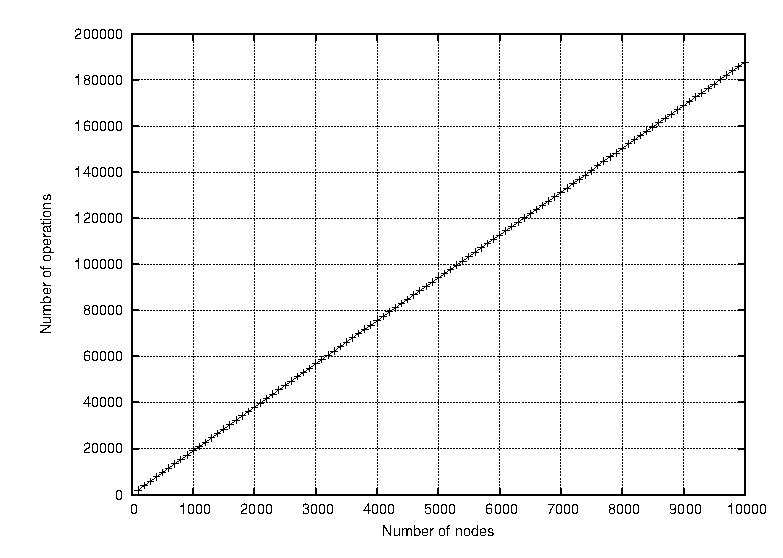
\includegraphics[width=12cm]{experiment.eps}

 \caption{Number of operations performed by Algorithm {\sc Subtree-Repeats}, according to the size of the input tree}
\label{fig:exp}
\end{figure}



\section{Conclusion and Further Work}\label{sec:conclusion}

In this report, we have provided 
a linear-time algorithm for computing all left seeds and all right seeds of a string, 
a linear-time algorithm for computing the mimimum left-seed array of a string, 
a linear-time solution for computing the maximum left-seed array of a string,
an $\cO(n\log n)$-time algorithm for the computing the minimum right-seed array of a string, 
and a linear-time solution for computing the maximum right-seed array of a string. 

Recently, Crochemore, Iliopoulos, Pissis and Tischler in \cite{CIPT10},
provided linear-time algorithms for checking the validity of minimal and maximal cover arrays
and inferring strings from valid minimal and maximal cover arrays.
Their result completed the series of algorithmic characterizations
of data structures that store fundamental features of strings.
They concern Border arrays \cite{DLL05jalc,FGLRSSY02} and Prefix arrays \cite{CCR09-pref}
that store periods of all the prefixes of a string, as well as the element
of Suffix arrays \cite{BannaiIST03,FS06} that memorizes the list of positions
of lexicographically sorted suffixes of the string.
The algorithms may be regarded as reverse engineering processes and, beyond their
obvious theoretical interest, they are useful to test the validity of some
constructions.

Hence, further work can be done on the following relevant problems as well.
%
\begin{problem}[Validity problem]
Let $A$ be an integer array of length $n$. Decide if $A$ is the minimal left (resp. right) seed array of some string.
\end{problem}
%
\begin{problem}[Construction Problem]
Let $A$ be an integer array of length $n$. When $A$ is a valid minimal left-seed (resp. right-seed) array, exhibit a string over an unbounded
alphabet whose minimal left-seed (resp. right-seed) array is $A$.
\end{problem}

Furthermore we have formally defined the problem of computing all the subtree 
repeats in ordered ranked trees and presented a new solution based on the bottom-up
technique. The proposed algorithm is divided into two phases: the preprocessing phase
and the phase where all the repeating subtrees are computed. The preprocessing
phase tranforms the given tree to a string representing its postfix notation, and
then computes and stores some useful properties of the tree. The second phase, for 
computing all the repeating subtrees, is done in a bottom-up manner, using a 
partitioning procedure. 

It is important to mention that the proposed algorithm for computing
all the subtree repeats in ordered ranked trees runs in linear time and space.
This problem is analogous to the well-known problem of finding all the repetitions in a given word.
The significance of the proposed algorithm is underlined by the fact that it can be applied in both
unlabelled and labelled ordered ranked trees. The presented experimental results
demonstrate the efficiency of the proposed algorithm in practice.

The goal of our future research is to modify and apply the proposed algorithm, as an alternative solution, 
on the maximum agreement subtree problem for trees representing the evolutionary history of 
a set of species.


\newpage
\bibliographystyle{abbrv}
\bibliography{BIB}

\newpage
\appendix

\section{Additional details for the Subtree repeats problem}
In this section more details on the solution of the Subtree repeats problem are given. In particular we show the procedures of the preprocessing phase, an example for the unlabelled case and the procedures for solving the labelled version of the problem.

\subsection{Preprocessing phase}
In this subsection, the procedures of the preprocessing phase are presented.


\begin{algorithm}\label{alg height}
%\caption{\textsc{Compute-Subtree-Height}}
\begin{algorithmic}[1]
\REQUIRE{{\sc Compute-Subtree-Height}($\varphi,n$)}
\STATE{$S \leftarrow \emptyset$};
\FOR{$i \leftarrow 1$ to $n$}
        \IF{$\varphi[i]=0$}
          \STATE{$Push( S, 0 )$};
          \STATE{$H[i] \leftarrow 0$};
        \ELSE
         \STATE{$r \leftarrow 0$};
         \FOR{$j \leftarrow 1$ to $\varphi[i]$}
           \STATE{$r \leftarrow \max ( r, Pop(S) )$};
         \ENDFOR
         \STATE{$H[i] \leftarrow r + 1$};
         \STATE{$Push(S,r + 1 )$};
        \ENDIF
\ENDFOR
\RETURN {Array $H[1\ldots n]$};
\end{algorithmic}
\end{algorithm}





\begin{algorithm}\label{alg parent}
%\caption{\textsc{Compute-Node-Parents}}
\begin{algorithmic}[1]
\REQUIRE{{\sc Compute-Node-Parents}($\varphi,n$)}
\STATE{$S \leftarrow \emptyset$};
\FOR{$i \leftarrow 1$ to $n$}
  \FOR{$j \leftarrow 1$ to $\varphi[i]$}
    \STATE{$r \leftarrow Pop(S)$};
    \STATE{$P[r] \leftarrow i$};
  \ENDFOR
  \STATE{$Push(S,i)$};
\ENDFOR
\RETURN {Array $P[1\ldots n-1]$};
\end{algorithmic}
\end{algorithm}

\begin{algorithm}\label{alg FC}
%\caption{\textsc{First-Child}}
\begin{algorithmic}[1]
\REQUIRE{{\sc First-Child}($\varphi,n$)}
\STATE{$S \leftarrow \emptyset$};
\FOR{$i \leftarrow 1$ to $n$}
        \IF{$\varphi[i]=0$}
          \STATE{$Push ( S, i )$};
        \ELSE
         \FOR{$j \leftarrow 1$ to $\varphi[i]-1$}
           \STATE{$r \leftarrow Pop(S)$};
           \STATE{$FC[r] \leftarrow 0$};
         \ENDFOR
         \STATE{$r \leftarrow Pop(S)$};
         \STATE{$FC[r] \leftarrow 1$};
         \STATE{$ Push(S,i)$};
        \ENDIF
\ENDFOR
\STATE$FC[n] \leftarrow 1$
\RETURN {Array $FC[1\ldots n]$};
\end{algorithmic}
\end{algorithm}
$\;$\\

\newpage


\subsection{Example}
In this subsection, we show how the proposed algorithm computes all the subtree repeats of the tree in Fig.~\ref{fig:tree}.

\begin{table}{
 \begin{center}
  \begin{tabular}{|@{}l@{}|@{}l@{}|@{}l@{}|@{}l@{}|@{}l@{}|@{}l@{}|@{}l@{}|@{}l@{}|@{}l@{}|@{}l@{}|@{}l@{}|@{}l@{}|@{}l@{}|@{}l@{}|@{}l@{}|@{}l@{}|@{}l@{}|@{}l@{}|@{}l@{}|@{}l@{}|@{}l@{}|@{}l@{}|@{}l@{}|@{}l@{}|@{}l@{}|@{}l@{}|}\hline
   index & 1 & 2 & 3 & 4 & 5 & 6 & 7 & 8 & 9 & 10 & 11 & 12 & 13 & 14 & 15 & 16 & 17 & 18 & 19 & 20 & 21 & 22 & 23 & 24 & 25\\\hline
   $post(t)$ & $a_{0}$ & $a_{0}$ & $a_{0}$ & $a_{1}$ & $a_{2}$ & $a_{0}$ & $a_{1}$ & $a_{3}$ & $a_{0}$ & $a_{1}$ & $a_{1}$ & $a_{1}$ & $a_{0}$ & $a_{0}$ & $a_{1}$ & $a_{2}$ & $a_{2}$ & $a_{0}$ & $a_{0}$ & $a_{2}$ & $a_{0}$ & $a_{0}$ & $a_{1}$ & $a_{2}$ & $a_{4}$\\\hline
   P   & 8 & 5 & 4 & 5 & 8 & 7 & 8 & 25 & 10 & 11 & 12 & 17 & 16 & 15 & 16 & 17 & 25 & 20 & 20 & 25 & 24 & 23 & 24 & 25 & -\\\hline
   H   & 0 & 0 & 0 & 1 & 2 & 0 & 1 & 3 & 0 & 1 & 2 & 3 & 0 & 0 & 1 & 2 & 4 & 0 & 0 & 1 & 0 & 0 & 1 & 2 & 5\\\hline
   FC  & 1 & 1 & 1 & 0 & 0 & 1 & 0 & 1 & 1 & 1 & 1 & 1 & 1 & 1 & 0 & 0 & 0 & 1 & 0 & 0 & 1 & 1 & 0 & 0 & -\\\hline
 \end{tabular}
\caption{Preprocessing output}
\end{center}
		}
		
	\end{table}



\begin{landscape}





\begin{scriptsize}$
\psmatrix[colsep=0.1,rowsep=0.2cm]
\text{Level 0}&&&&\{1,2,3,6,9,13,14,18,19,21,22\}_{\underline{a_{0}}}\\
\text{Level 1}&&\{3,6,9,14,18,22\}_{a_{0}}\\
&\{3,6,9,14,22\}_{\underline{a_{0}a_{1}}}&&\{18\}_{a_{0}a_{0}}\\
&&&\{18\}_{\underline{a_{0}a_{0}a_{2}}}\\
\text{Level 2}&\{9\}_{a_{0}a_{1}}&&&\{2,13,21\}_{a_{0}}\\
&\{9\}_{\underline{a_{0}a_{1}a_{1}}}&&&\{2,13,21\}_{a_{0}a_{0}}\\
&&&&\{2,13,21\}_{a_{0}a_{0}a_{1}}\\
&&&&\{2,13,21\}_{\underline{a_{0}a_{0}a_{1}a_{2}}}\\
\text{Level 3}&\{9\}_{a_{0}a_{1}a_{1}}&&&&&\{1\}_{a_{0}}\\
&\{9\}_{\underline{a_{0}a_{1}a_{1}a_{1}}}&&&&&\{1\}_{a_{0}a_{0}a_{0}a_{1}a_{2}}\\
&&&&&&\{1\}_{a_{0}a_{0}a_{0}a_{1}a_{2}a_{0}a_{1}}\\
&&&&&&\{1\}_{\underline{a_{0}a_{0}a_{0}a_{1}a_{2}a_{0}a_{1}a_{3}}}\\
\text{Level 4}&\{9\}_{a_{0}a_{1}a_{1}a_{1}}\\
&\{9\}_{a_{0}a_{1}a_{1}a_{1}a_{0}a_{0}a_{0}a_{1}a_{2}}\\
&\{9\}_{\underline{a_{0}a_{1}a_{1}a_{1}a_{0}a_{0}a_{0}a_{1}a_{2}a_{2}}}\\
\text{Level 5}&&&&&&\{1\}_{a_{0}a_{0}a_{0}a_{1}a_{2}a_{0}a_{1}a_{3}}\\
&&&&&&\{1\}_{a_{0}a_{0}a_{0}a_{1}a_{2}a_{0}a_{1}a_{3}a_{0}a_{1}a_{1}a_{1}a_{0}a_{0}a_{0}a_{1}a_{2}a_{2}}\\
&&&&&&\{1\}_{a_{0}a_{0}a_{0}a_{1}a_{2}a_{0}a_{1}a_{3}a_{0}a_{1}a_{1}a_{1}a_{0}a_{0}a_{0}a_{1}a_{2}a_{2}a_{0}a_{0}a_{2}a_{0}a_{0}a_{0}a_{1}a_{2}}\\
&&&&&&\{1\}_{\underline{a_{0}a_{0}a_{0}a_{1}a_{2}a_{0}a_{1}a_{3}a_{0}a_{1}a_{1}a_{1}a_{0}a_{0}a_{0}a_{1}a_{2}a_{2}a_{0}a_{0}a_{2}a_{0}a_{0}a_{0}a_{1}a_{2}a_{4}}}\\
\ncline{->}{1,5}{2,3}\ncline{->}{1,5}{5,5}\ncline{->}{1,5}{9,7}
\ncline{->}{2,3}{3,2}\ncline{->}{2,3}{3,4}
\ncline{->}{3,2}{5,2}\ncline{->}{3,4}{4,4}
\ncline{->}{5,2}{6,2}\ncline{->}{5,5}{6,5}
\ncline{->}{6,2}{9,2}\ncline{->}{6,5}{7,5}
\ncline{->}{7,5}{8,5}
\ncline{->}{9,2}{10,2}\ncline{->}{9,7}{10,7}
\ncline{->}{10,2}{13,2}\ncline{->}{10,7}{11,7}
\ncline{->}{13,2}{14,2}\ncline{->}{11,7}{12,7}
\ncline{->}{14,2}{15,2}\ncline{->}{12,7}{16,7}
\ncline{->}{16,7}{17,7}
\ncline{->}{17,7}{18,7}
\ncline{->}{18,7}{19,7}
\ncline{->}{19,7}{20,7}
%\ncarc[arcangle=-30]{<-}{1,1}{2,2}
\endpsmatrix
$\end{scriptsize}
\end{landscape}


	\begin{table}{
\begin{center}
			\begin{tabular}{|l|l|}\hline
                                 index & Sets\\  \hline
				   $0$ & $\{1,2,3,6,9,13,14,18,19,21,22\}_{1}$\\  
				   $1$ & $\{3,6,9,14,18,22\}_{1}$\\
				   $2$ & $\{9\}_{2},\{2,13,21\}_{1}$\\
				   $3$ & $\{9\}_{3},\{1\}_{1}$ \\
				   $4$ & $\{9\}_{4}$\\
				   $5$ & $\{1\}_{8}$\\\hline
			\end{tabular}
               \caption{Level array}
\end{center}

		}
		
	\end{table}
	\begin{table}{
\begin{center}
			\begin{tabular}{|l|l|}\hline
                                 index & Factors of subtrees\\  \hline
                                   $1$ & $a_{0}$\\ 
				   $2$ & $a_{0}a_{0}a_{2}$\\
				   $3$ & $a_{0}a_{1}$\\
				   $4$ & $a_{0}a_{0}a_{1}a_{2}$ \\
				   $5$ & $a_{0}a_{1}a_{1}$\\
				   $6$ & $a_{0}a_{0}a_{0}a_{1}a_{2}a_{0}a_{1}a_{3}$\\
				   $7$ & $a_{0}a_{1}a_{1}a_{1}$\\
				   $8$ & $a_{0}a_{1}a_{1}a_{1}a_{0}a_{0}a_{0}a_{1}a_{2}a_{2}$\\
				   $9$ & $a_{0}a_{0}a_{0}a_{1}a_{2}a_{0}a_{1}a_{3}a_{0}a_{1}a_{1}a_{1}a_{0}a_{0}a_{0}a_{1}a_{2}a_{2}a_{0}a_{0}a_{2}a_{0}a_{0}a_{0}a_{1}a_{2}a_{4}$\\ \hline
			\end{tabular}
               \caption{Indexing of subtrees}
\end{center}

		}
		
	\end{table}

\subsection{Procedures for labelled ordered ranked trees}
In this subsection, the procedures for computing all the subtree repeats of a given labelled ordered rank tree are given.


\begin{algorithm}
%\caption{\textsc{Partitioning-L}}
\begin{algorithmic}[1]
\REQUIRE{{\sc Partitioning-L}($E$)}
\FOR{$i\in S$}
 \STATE{$next=i+\ell_{E}$};
   \IF{$T[next]\neq 0$}
    \STATE{$E_{T[next]} \leftarrow  (S_{T[next]}\bigcup \{i\},\ell_{E}+TL[next],ac_{E}-1) $};
   \ELSE
    \STATE{$E_{\varphi(post(t)[next])} \leftarrow  (S_{\varphi(post(t)[next])}\bigcup \{i\},\ell_{E}+1,ac_{E}-1+\varphi[next] ) $};
   \ENDIF
\ENDFOR
\FOR{every $class$ created in the second step of the above loop}
 \FOR{$i\in S_{class}$}
  \STATE{$next=i+\ell_{E_{class}}-1$};
  \STATE{$E_{label(post(t)[next]), class} \leftarrow  (S_{label(post(t)[next]), class}\bigcup \{i\},\ell_{E_{class}},ac_{E_{class}}) $};
 \ENDFOR
\ENDFOR
\FOR{every $class$ considered}
 \IF{$ac_{class}=0$}
  \STATE{Output $S_{class}$, $\ell_{class}$};
  \STATE{$sc=sc+1$};
  \FOR{$i\in S_{class}$}
   \STATE{$T[i] \leftarrow sc$};
   \STATE{$TL[i] \leftarrow \ell[E_{class}]$};
  \ENDFOR
  \STATE{Assign level($E_{class}$)};
 \ELSE
  \STATE{Partitioning($E_{class}$)};
 \ENDIF
\ENDFOR
\RETURN {Partitioning of E in classes corresponding to next element to be considered};
\end{algorithmic}
\end{algorithm}


\begin{algorithm}
%\caption{\textsc{Subtree-Repeats-L}}
\begin{algorithmic}[1]
\REQUIRE{{\sc Subtree-Repeats-L}($post(t), FC, P, H, n, \varphi$)}
\STATE{$sc \leftarrow 1$}; 
\FOR{$i \leftarrow 1$ to $n$}
 \IF{$\varphi(post(t)[i])=0$}
  \STATE{$E_{label(post(t)[i])} \leftarrow  (S_{label(post(t)[i])}\bigcup \{i\},1,0) $};
  \STATE{$T[i] \leftarrow sc$};
  \STATE{$TL[i] \leftarrow 1$}; 
 \ELSE
  \STATE{$T[i] \leftarrow 0$};
  \STATE{$TL[i] \leftarrow 0$};
 \ENDIF
\ENDFOR
\FOR{every $class$ considered}
 \STATE{Output $S_{class}$, $1$};
 \STATE{$sc=sc+1$};
 \STATE{Assign level($E_{class}$)};
\ENDFOR
\FOR{$i \leftarrow 1$ to $H[n]$}
 \WHILE{LA[i] non empty}
  \STATE{$E \leftarrow pop(LA[i])$};
  \STATE{Partition E};
 \ENDWHILE
\ENDFOR
\RETURN {Sets of starting positions of Subtrees in post(t) together with their length};
\end{algorithmic}
\end{algorithm}




 
%% The Appendices part is started with the command \appendix;
%% appendix sections are then done as normal sections
%% \appendix

%% \section{}
%% \label{}

%% References
%%
%% Following citation commands can be used in the body text:
%% Usage of \cite is as follows:
%%   \cite{key}          ==>>  [#]
%%   \cite[chap. 2]{key} ==>>  [#, chap. 2]
%%   \citet{key}         ==>>  Author [#]

%% References with bibTeX database:



%% Authors are advised to submit their bibtex database files. They are
%% requested to list a bibtex style file in the manuscript if they do
%% not want to use model1-num-names.bst.

%% References without bibTeX database:

% \begin{thebibliography}{00}

%% \bibitem must have the following form:
%%   \bibitem{key}...
%%

% \bibitem{}

% \end{thebibliography}

\end{document}

%%
%% End of file `elsarticle-template-1-num.tex'.
